\chapter{In-depth Contrastive Error Analysis}
\label{chap:analysis}

% Length
% Graph factors
% Linguistic factors

% Peking: Ensemble method, combination of transition-based and graph-based
% Turku: Support Vector Machines
% Lisbon: A graph algorithm

In this chapter we present an in-depth contrastive error analysis of the results of SemEval-2015 for the Peking, Turku and Lisbon system submissions described in Chapter \ref{chap:semantic}. There where 6 submissions to SemEval-2015, including an `in-official' submission by a sub-set of the task organizers. We have made the choice of focusing on three of these parsing systems in our analysis. This is based on three criteria:

\begin{enumerate}
    \item The chosen systems must have the highest overall scores in SemEval-2015.
    \item The technical approach of the three parsing systems must be different from one another: both the local transition-based and global graph-based models that we examined in Chapter \ref{chap:background} must be represented.
    \item When choosing between submissions where similar technical approach are utilised, we must exclude the system with the overall lowest accuracy score.
\end{enumerate}

The aim of our in-depth contrastive error analysis is to gain insights into the state-of-the-art in semantic dependency parsing. The study is performed in order to:

\begin{enumerate}
    \item Find similarities and differences in the results among a chosen set of parsing systems in order to compare and contrast their strengths and weaknesses.
    \item Empirically identify and verify which types of errors that can be the focus of future research on improving the accuracy of the state-of-the-art in semantic dependency parsing.
    \item Examine the possibility of using the results of our study to modify and improve upon an existing system, or create a new system, in order to push the envelope on the accuracy of semantic dependency parsing.
\end{enumerate}

% We will argue that the analysis presented in this chapter can highlight the correlation between the specific types of errors that these parsers make and their theoretical foundation. The analysis presented is thus based on the general knowledge of the parsing systems, as described in Chapter \ref{chap:semantic}, and the specific observations made in our analysis of their results from SemEval-2015.

In our analysis we draw inspiration from three similar studies by \citeA{McD:Niv:07}, \citeA{McD:Niv:11}, and \citeA{Choi:Tetreaul:Stent:15}. In these studies a comparative analysis of a set of syntactic parsers is presented where various types of errors are highlighted. The first and second study focus on three types of errors: (1) length factors, (2) graph factors, and (3) linguistic factors. The third study, in addition to these three factors, also examine the time complexity of parsing systems: where both training and parsing time is taken into consideration. We will structure our analysis in a similar fashion, but exclude time complexity, and include the multi-classification task of frame predication introduced in SemEval-2015.

In addition to narrowing down the scope in terms of choosing three parsing systems, we also exclude results for the PAS target representation. The reasoning behind this is that the DM and PAS target representations are relatively similar. Examining Table \ref{fig:data} in Chapter \ref{chap:semantic}, we observe that DM and PAS are close to identical in the number of labels, percentage of graphs being trees, and percentage of dependencies being projective. The major difference between the two target representations is the percentage of so-called singletons, i.e. nodes not connected to any other node in the dependency graph. The DM target representation has approximately 5 times as many singletons as PAS. With the exception of singletons, we assume that our analysis of the DM results will yield similar results as PAS. This hypothesis was confirmed by running the error analysis on the PAS target representation, and observing that for most types of errors there is a strong correlation in the types of errors made when using the DM target representation for training and testing.

Before embarking on our in-depth contrastive error analysis, we examine overall statistics on the three parsing systems.

\section{Overall Accuracy}

\begin{table}
    \centering
    \begin{tabular}{@{}cccccccccc@{}}
        \toprule
        \multicolumn{1}{c}{ }
        & \multicolumn{1}{c}{ }
        & \multicolumn{4}{c}{\textbf{DM}}
        & \multicolumn{4}{c}{\textbf{PSD}} \\
        \cmidrule(lr){3-6}
        \cmidrule(lr){7-10}
        &
        LF.av &
        LF & LP & LR & FF &
        LF & LP & LR & FF \\
        \midrule
        Peking & 85.33 & 89.09 & 90.93 & 87.32 & 63.08 & 75.66 & 78.60 & 72.93 & 49.95 \\
        Lisbon & 85.15 & 88.21 & 89.84 & 86.64 & 00.15 & 76.36 & 78.62 & 74.23 & 00.03 \\
        \midrule
        Lisbon* & 86.23 & 89.44 & 90.52 & 88.39 & 00.20 & 77.58 & 79.88 & 75.41 & 00.06 \\
        Turku* & 83.47 & 86.17 & 87.80 & 84.60 & 54.67 & 73.63 & 76.10 & 71.32 & 53.20 \\
        \bottomrule
        
        \\
        \toprule
        \multicolumn{1}{c}{ }
        & \multicolumn{1}{c}{ }
        & \multicolumn{4}{c}{\textbf{DM}}
        & \multicolumn{4}{c}{\textbf{PSD}} \\
        \cmidrule(lr){3-6}
        \cmidrule(lr){7-10}
        &
        LF.av &
        LF & LP & LR & FF &
        LF & LP & LR & FF \\
        \midrule
        Lisbon & 81.15 & 81.75 & 84.81 & 78.90 & 00.27 & 74.82 & 78.68 & 71.31 & 02.09 \\
        Peking & 80.78 & 81.84 & 84.29 & 79.53 & 47.49 & 73.28 & 77.36 & 69.61 & 34.28 \\
        \midrule
        Lisbon* & 82.53 & 83.77 & 85.79 & 81.84 & 00.35 & 76.18 & 80.12 & 72.61 & 02.25 \\
        Turku* & 78.85 & 79.01 & 81.54 & 76.63 & 39.15 & 71.59 & 74.92 & 68.55 & 38.75 \\
        \bottomrule
    \end{tabular}
    \caption{SemEval-2015 results from the closed track (unmarked) and open track (marked *) of the in-domain (top) and out-of-domain (bottom) data for the three parsers included our the analysis.}
    \label{fig:data:recap}
\end{table}

In Chapter \ref{chap:semantic} we reviewed the technical aspects of the three parsing systems we will examine here. The Peking system: an ensemble of transition-based and graph-based models, the Turku system: a combination of several classifiers for specific aspects of the semantic dependency graphs, and the Lisbon system: a graph-based feature-rich linear model that parametrize globally over first and second order dependencies.

In Table \ref{fig:data:recap} we can see the performance of the three parsing systems. An obvious aspect of the results is that the parsing systems perform better on the in-domain versus the out-of-domain data sets. This is to be expected, as data-driven parsing will yield better results on data that is within the domain of the training data. In our analysis we examine the results for the in-domain data. In terms of the specific types of errors we examine, the type specific errors: length, graph and linguistic factors, are quite evenly lower. So we expect the results of our analysis to be the same if we had chosen to sue the out-of-domain data sets.

The parsing could be run in an open and closed track, which we described in Chapter \ref{chap:semantic}. Lisbon is the only team that participated in both tracks, Peking only in the closed and Turku only in the open track.\footnote{Turku also participated in the gold track, as the only team, which we exclude from our analysis as it does not provide any addition to the comparative nature of our discussion.} For our analysis we have chosen to use data from the closed track for Lisbon and Peking, and since no data for the closed track exists for Turku, we use the results run in the open track. It is therefore important to note that the comparisons in our analysis must bear in mind that the data for Turku is from the open track, and that the additional use of syntactic parsing impacts the parsing results positively: see \citeA{Kanerva:Turku:15} for more details. This is something we observe in the results of the Lisbon parsing system, which has a higher accuracy in the open track compared to the closed track.

Examining Table \ref{fig:data:recap}, we see that the Peking parser performs slightly better than Lisbon on average. However, looking closer we see that the average increase is due to the higher scores for the DM target representation, and that the Lisbon parser performs better on the PSD target representation. On the out-of-domain data set the Lisbon parsing system scores higher. The Turku system, which only submitted results for the closed track, performs substantially lower than the Lisbon system.

The measures used for determining the scores of the submission are \textit{precision}, \textit{recall}, and \textit{f-score}. When calculating these, we use the measures \textit{true positives}: instances that have been correctly predicted, \textit{false positives}: instances that have been falsely identified, and \textit{false negatives}: instances that should have been predicted, but have not.

Precision, also known as positive predictive value, is a measure for the reliability of a system's predictions. These are the dependencies that have been correctly assigned when parsing. We calculate this as follows:

\begin{equation*}
    \text{Precision} = \frac{\text{true positives}}{\text{true positives + false positives}}
\end{equation*}

\vspace{1ex}

Recall, also known as sensitivity, is the measure for how robust a system is. These are the fraction of relevant dependencies that have been assigned at parsing. This measure is calculated as:

\begin{equation*}
    \text{Recall} = \frac{\text{true positives}}{\text{true positives + false
            negatives}}
\end{equation*}

\vspace{1ex}

F-score is the so-called \textit{harmonic mean} of the precision and recall, and is calculated as follows:

\begin{equation*}
    \text{F-score} = 2*\frac{\text{precision * recall}}{\text{precision + recall}}
\end{equation*}

\vspace{1ex}

We will now start our error analysis by first examining length factors.
    
\section{Length factors}

\begin{figure}[h]
    \centering
    \begin{minipage}{0.50\textwidth}
        \centering
        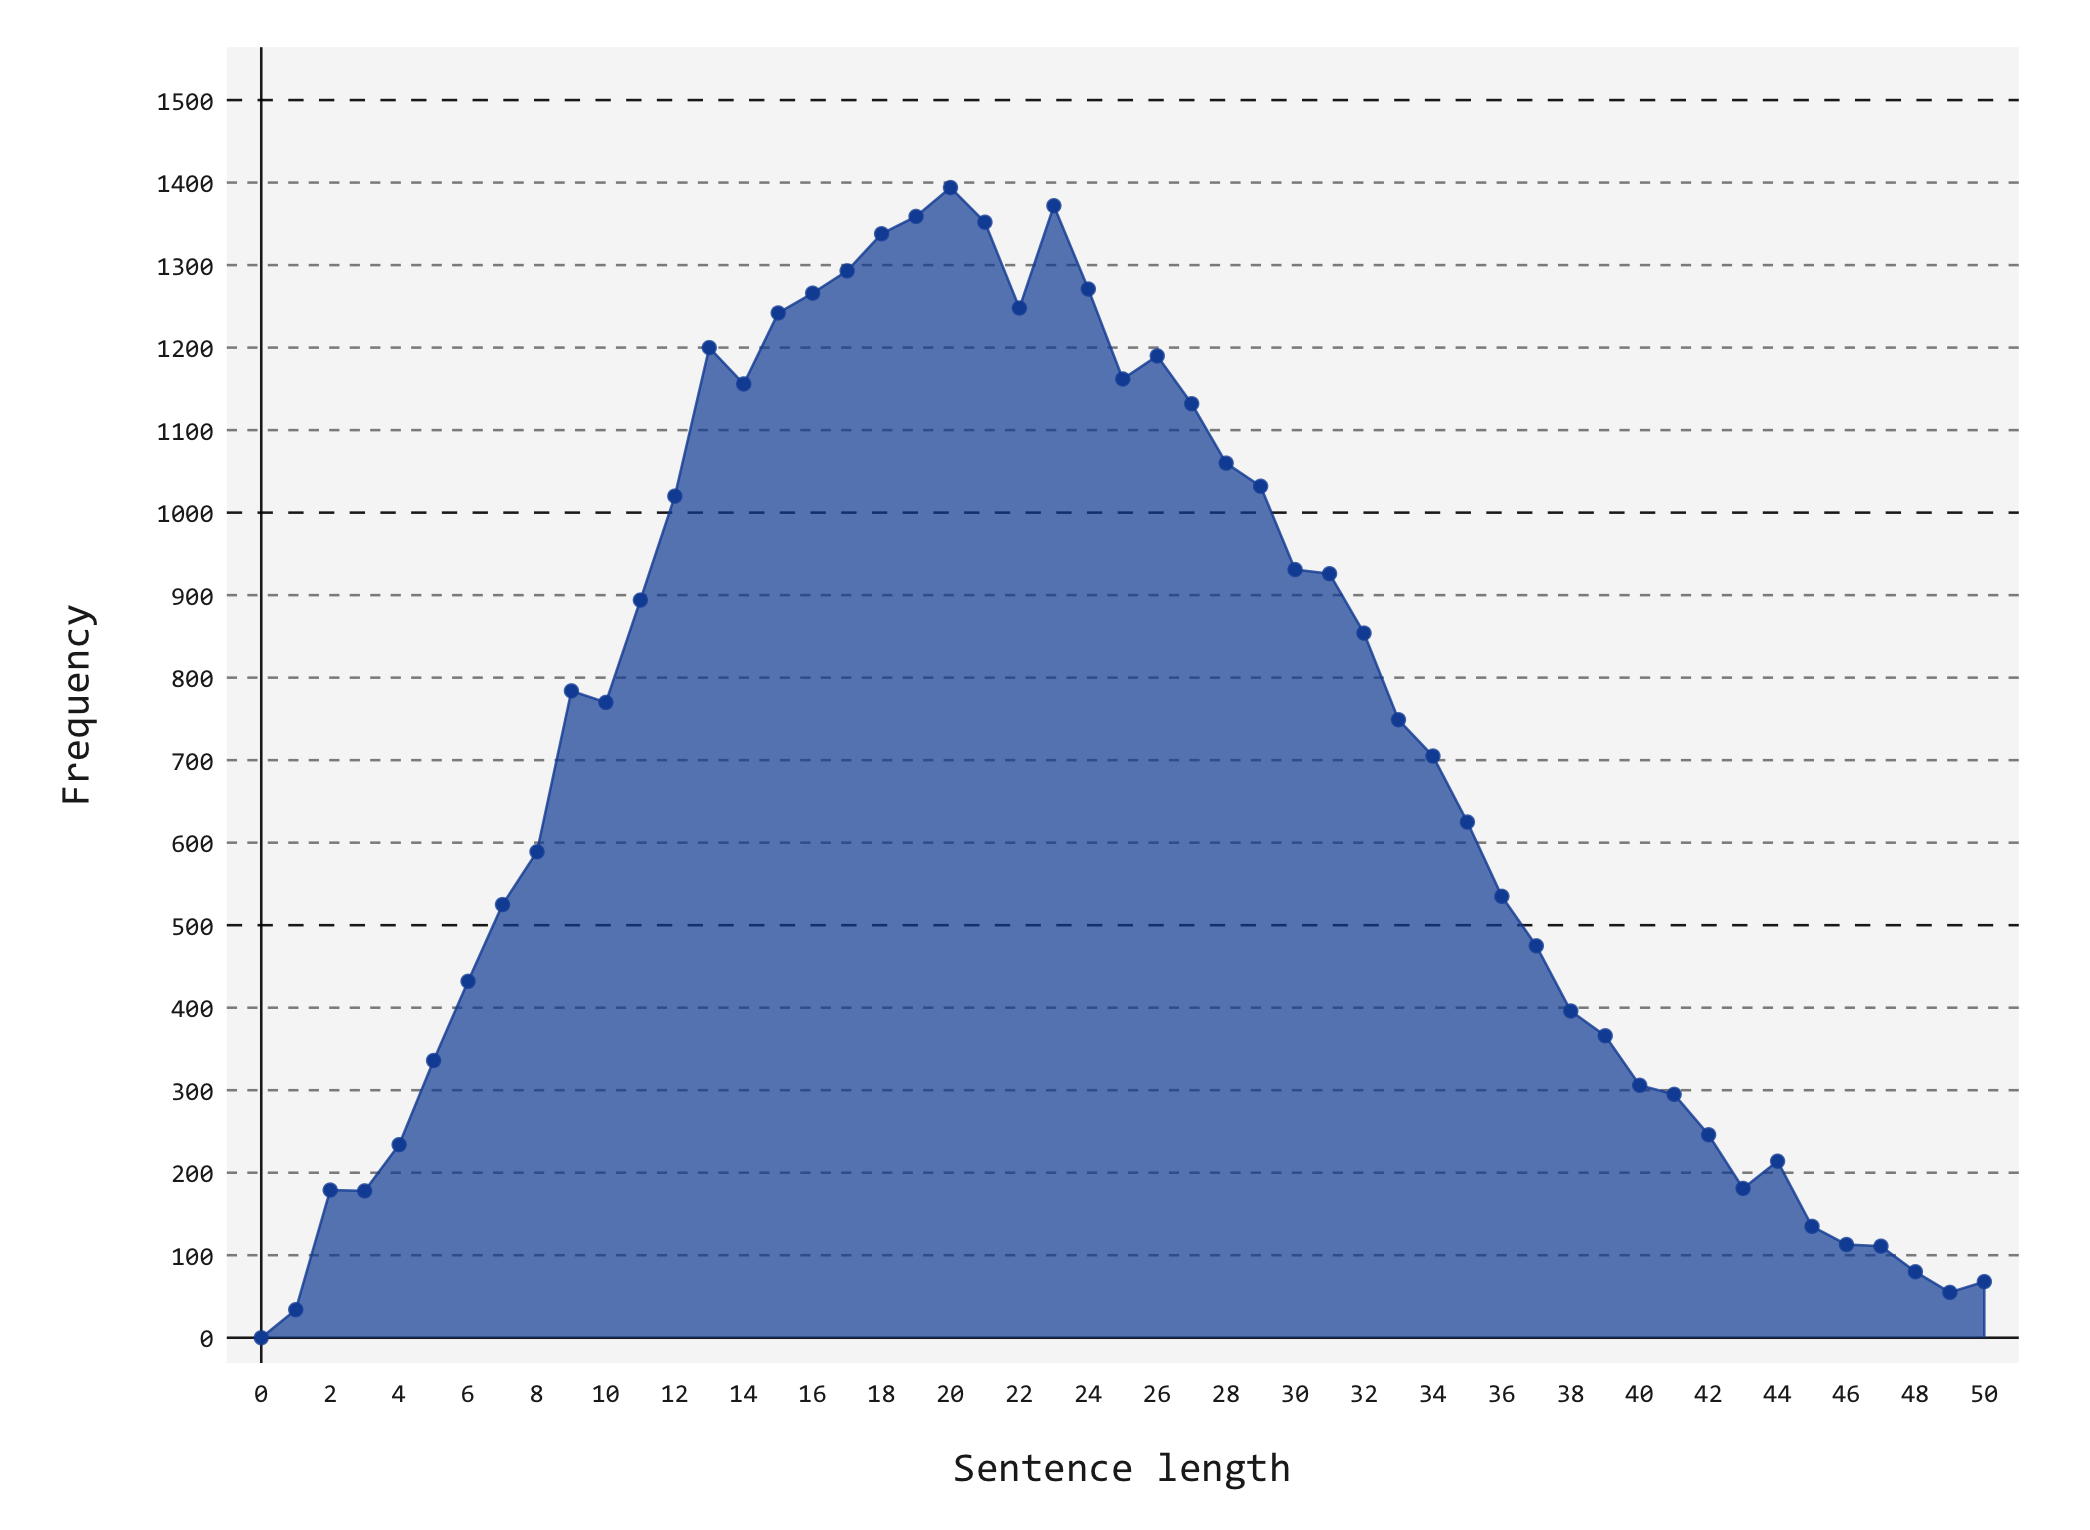
\includegraphics[width=\textwidth]{s_length_training}
    \end{minipage}\hfill
    \begin{minipage}{0.50\textwidth}
        \centering
        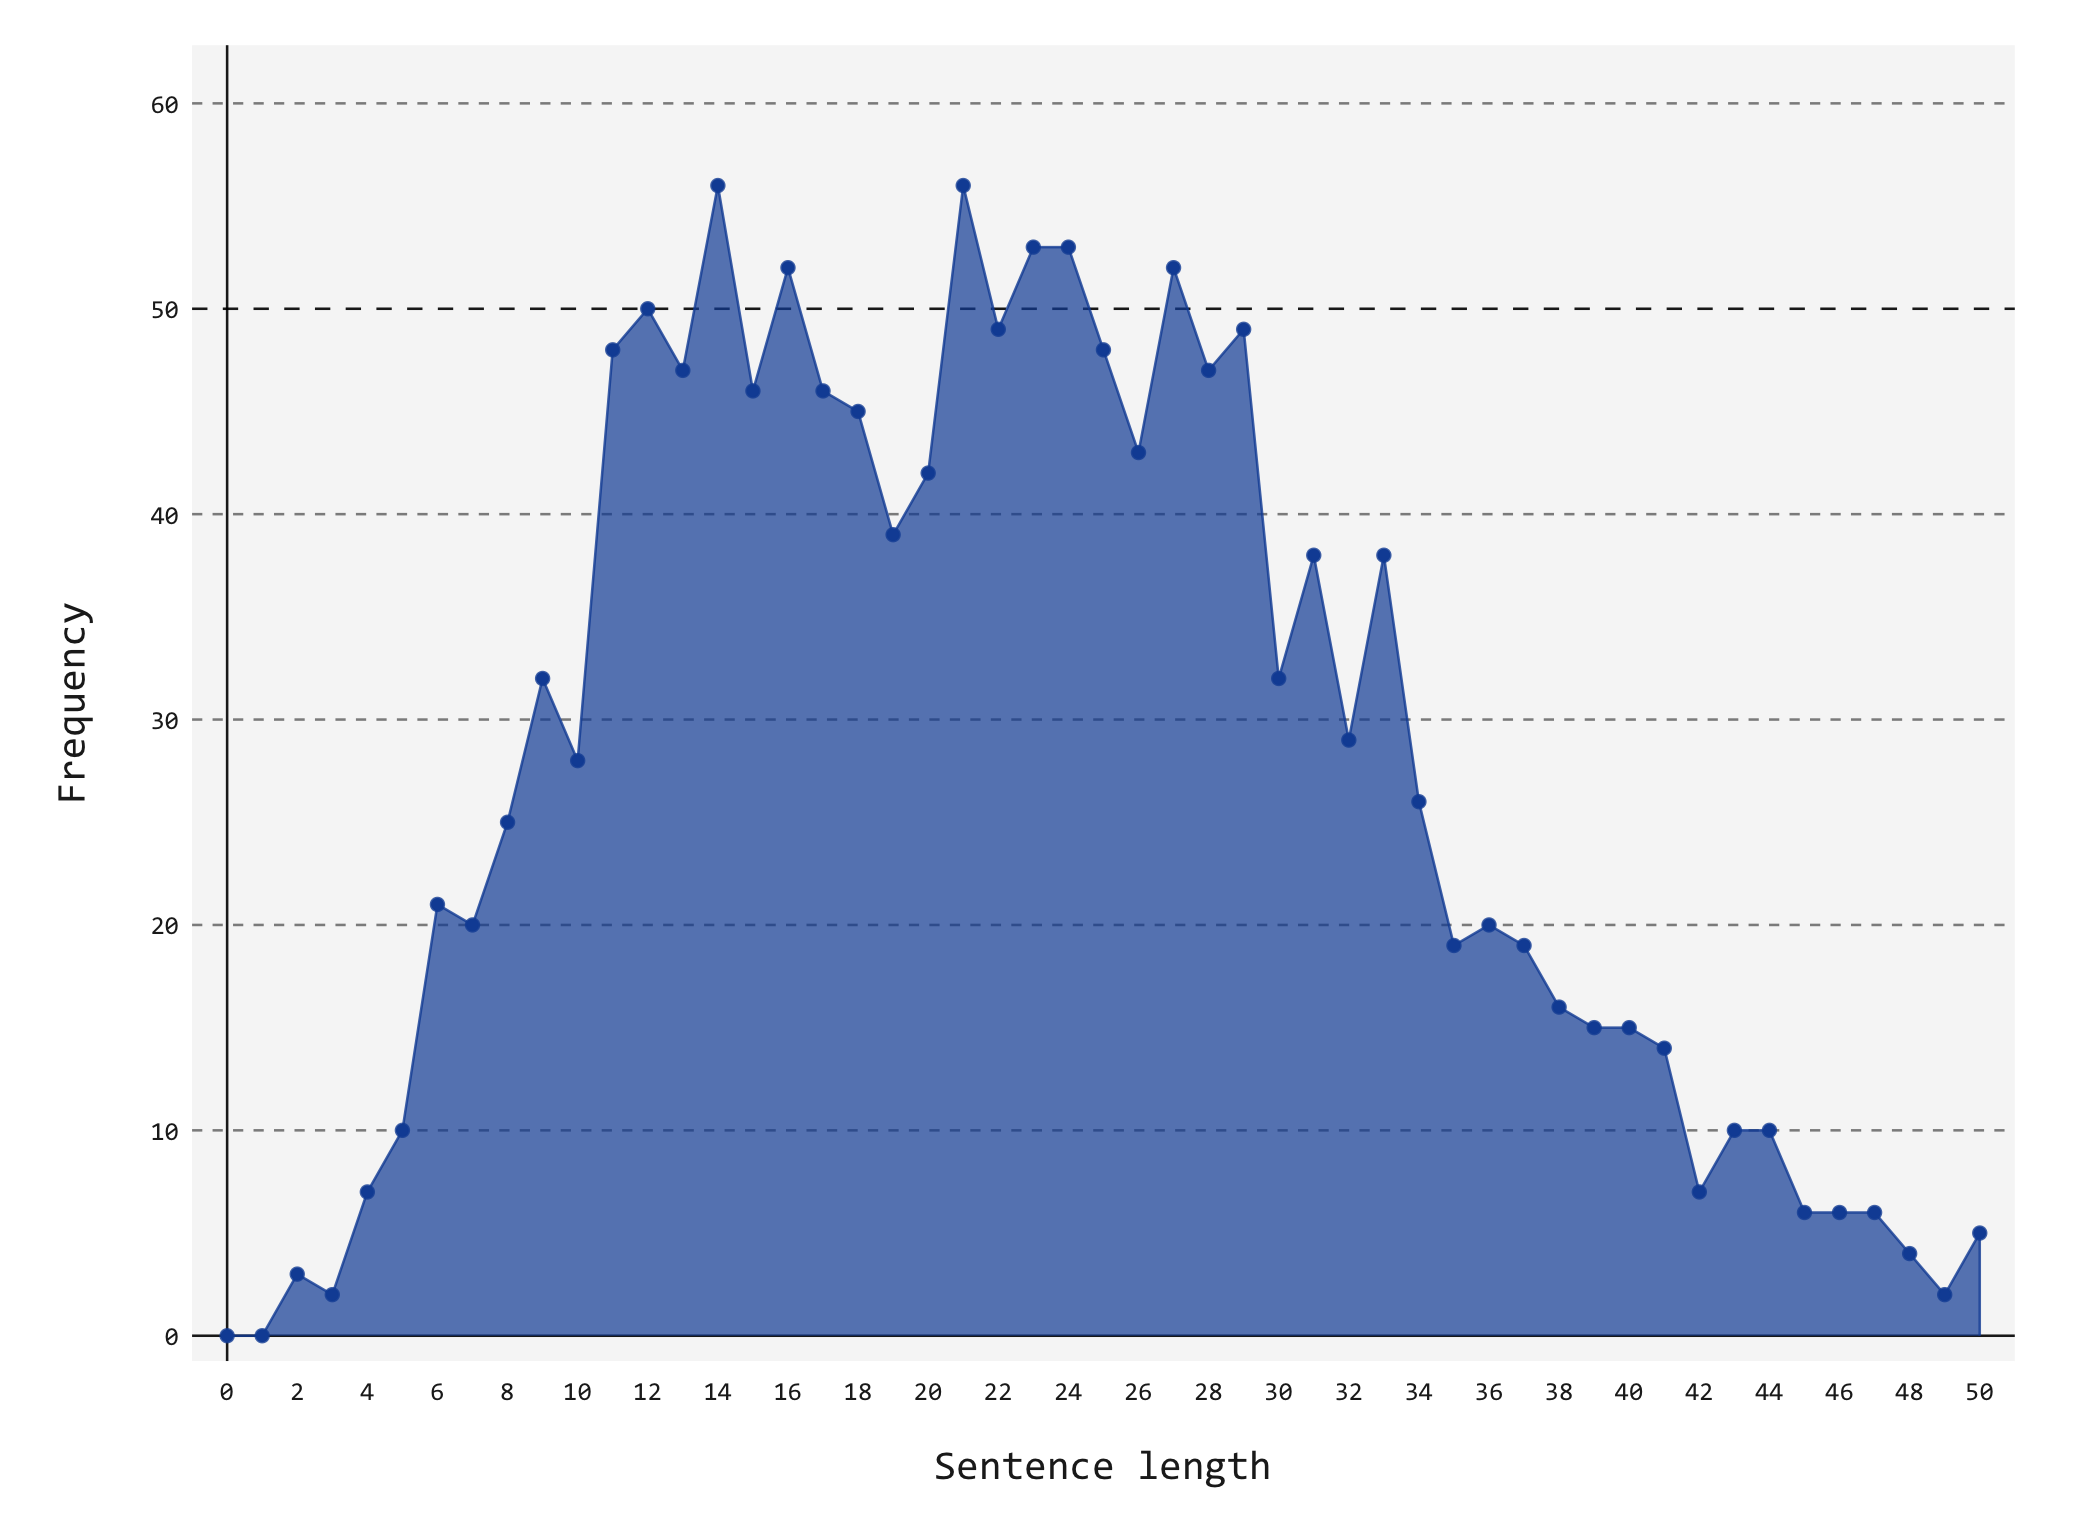
\includegraphics[width=\textwidth]{s_length_testing}
    \end{minipage}
    \caption{Distribution of sentence lengths and their frequency in the training (left) and test (right) data.}
    \label{fig:sentence_length}
\end{figure}

As \citeA{McD:Niv:07} point out, it is well known that syntactic parsing systems produce results with lower accuracy for longer sentences. We observe the same phenomena in the results of our three parsing systems. Parsing accuracy is correlated with sentence length. \citeA{McD:Niv:11} claims that this is primarily due to more complex constructions in longer sentences, such as prepositions, conjunctions, and multi-class sentences.

Another type of length factor is the length of dependencies, which also has an impact on the accuracy of predictions. We define the length of a dependency from word $w_i$ to $w_j$ as $j - i$. For the English language, and from examining the data sets used in SemEval-2015, we can generally state that short dependencies are modifiers of nouns, such as determiners, adjectives or pronouns. Longer dependencies are in most cases words that modify the main verb or root of the sentence. 

\subsection{Sentence length}

In this section we will examine sentence length as a factor of parsing. First we point out the distribution of sentence lengths in the training and test data in Figure \ref{fig:sentence_length}, which approximates the Bell curve. Average sentence length is 22.51 for the training, and 22.66 lexical units for the test data. It is worth noting that there are very few sentences that have a length below 3 lexical units in both the training and test data, and when we examine accuracy in relation to sentence length, we should exclude such outliers as these will inevitably produce low accuracy scores. 

In Figures \ref{fig:dm_s_length} and \ref{fig:psd_s_length}, we have graphs for the precision and recall of the three parsing systems for both the DM and SDP target representations. As \citeA{McD:Niv:07}, \citeA{McD:Niv:11}, and \citeA{Choi:Tetreaul:Stent:15} found when examining various syntactic parsers, there is also a correlation between sentence length and the accuracy of semantic dependency parsing systems. The longer the sentence, the lower the precision and recall of the results.

However, the trend is more prevalent for the PSD target representation than the DM. If we go back to Figure \label{fig:data} from Chapter \ref{chap:semantic}, we see that the PSD target representation has 91 labels, whereas DM has 59. This accounts for some of the reduction in precision and recall that we observe in the results on these two target representations.


% Sentence lengths
\begin{figure}[h]
    \centering
    \begin{minipage}{0.50\textwidth}
        \centering
        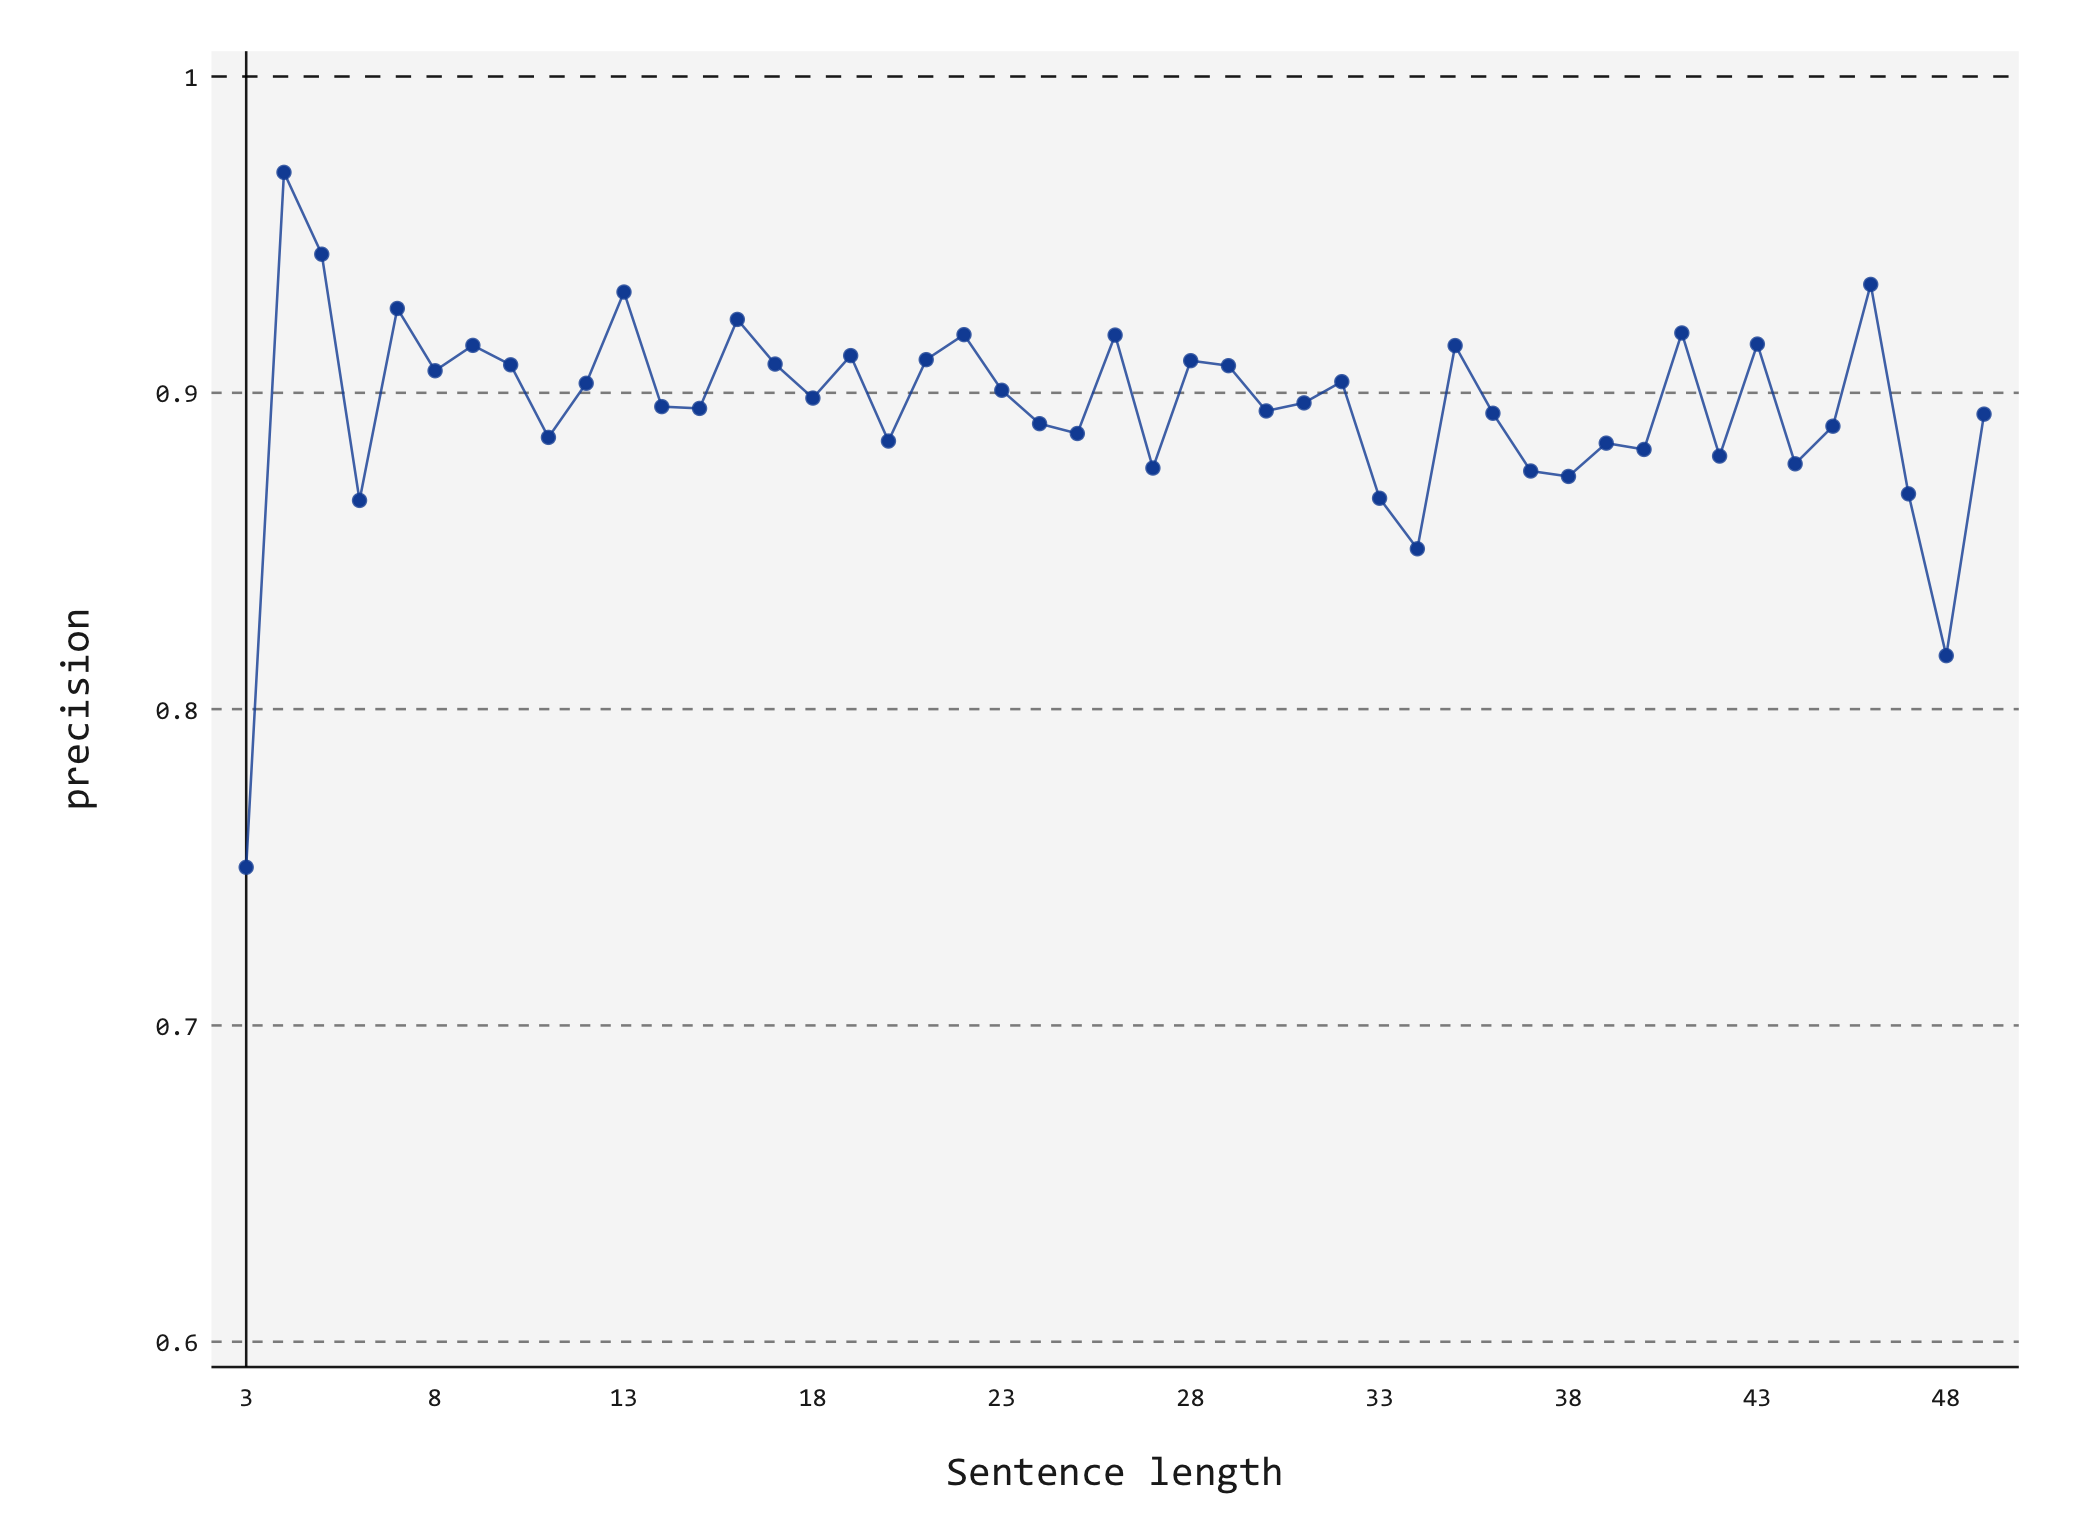
\includegraphics[width=\textwidth]{sentence_dm_lisbon_precision}
    \end{minipage}\hfill
    \begin{minipage}{0.50\textwidth}
        \centering
        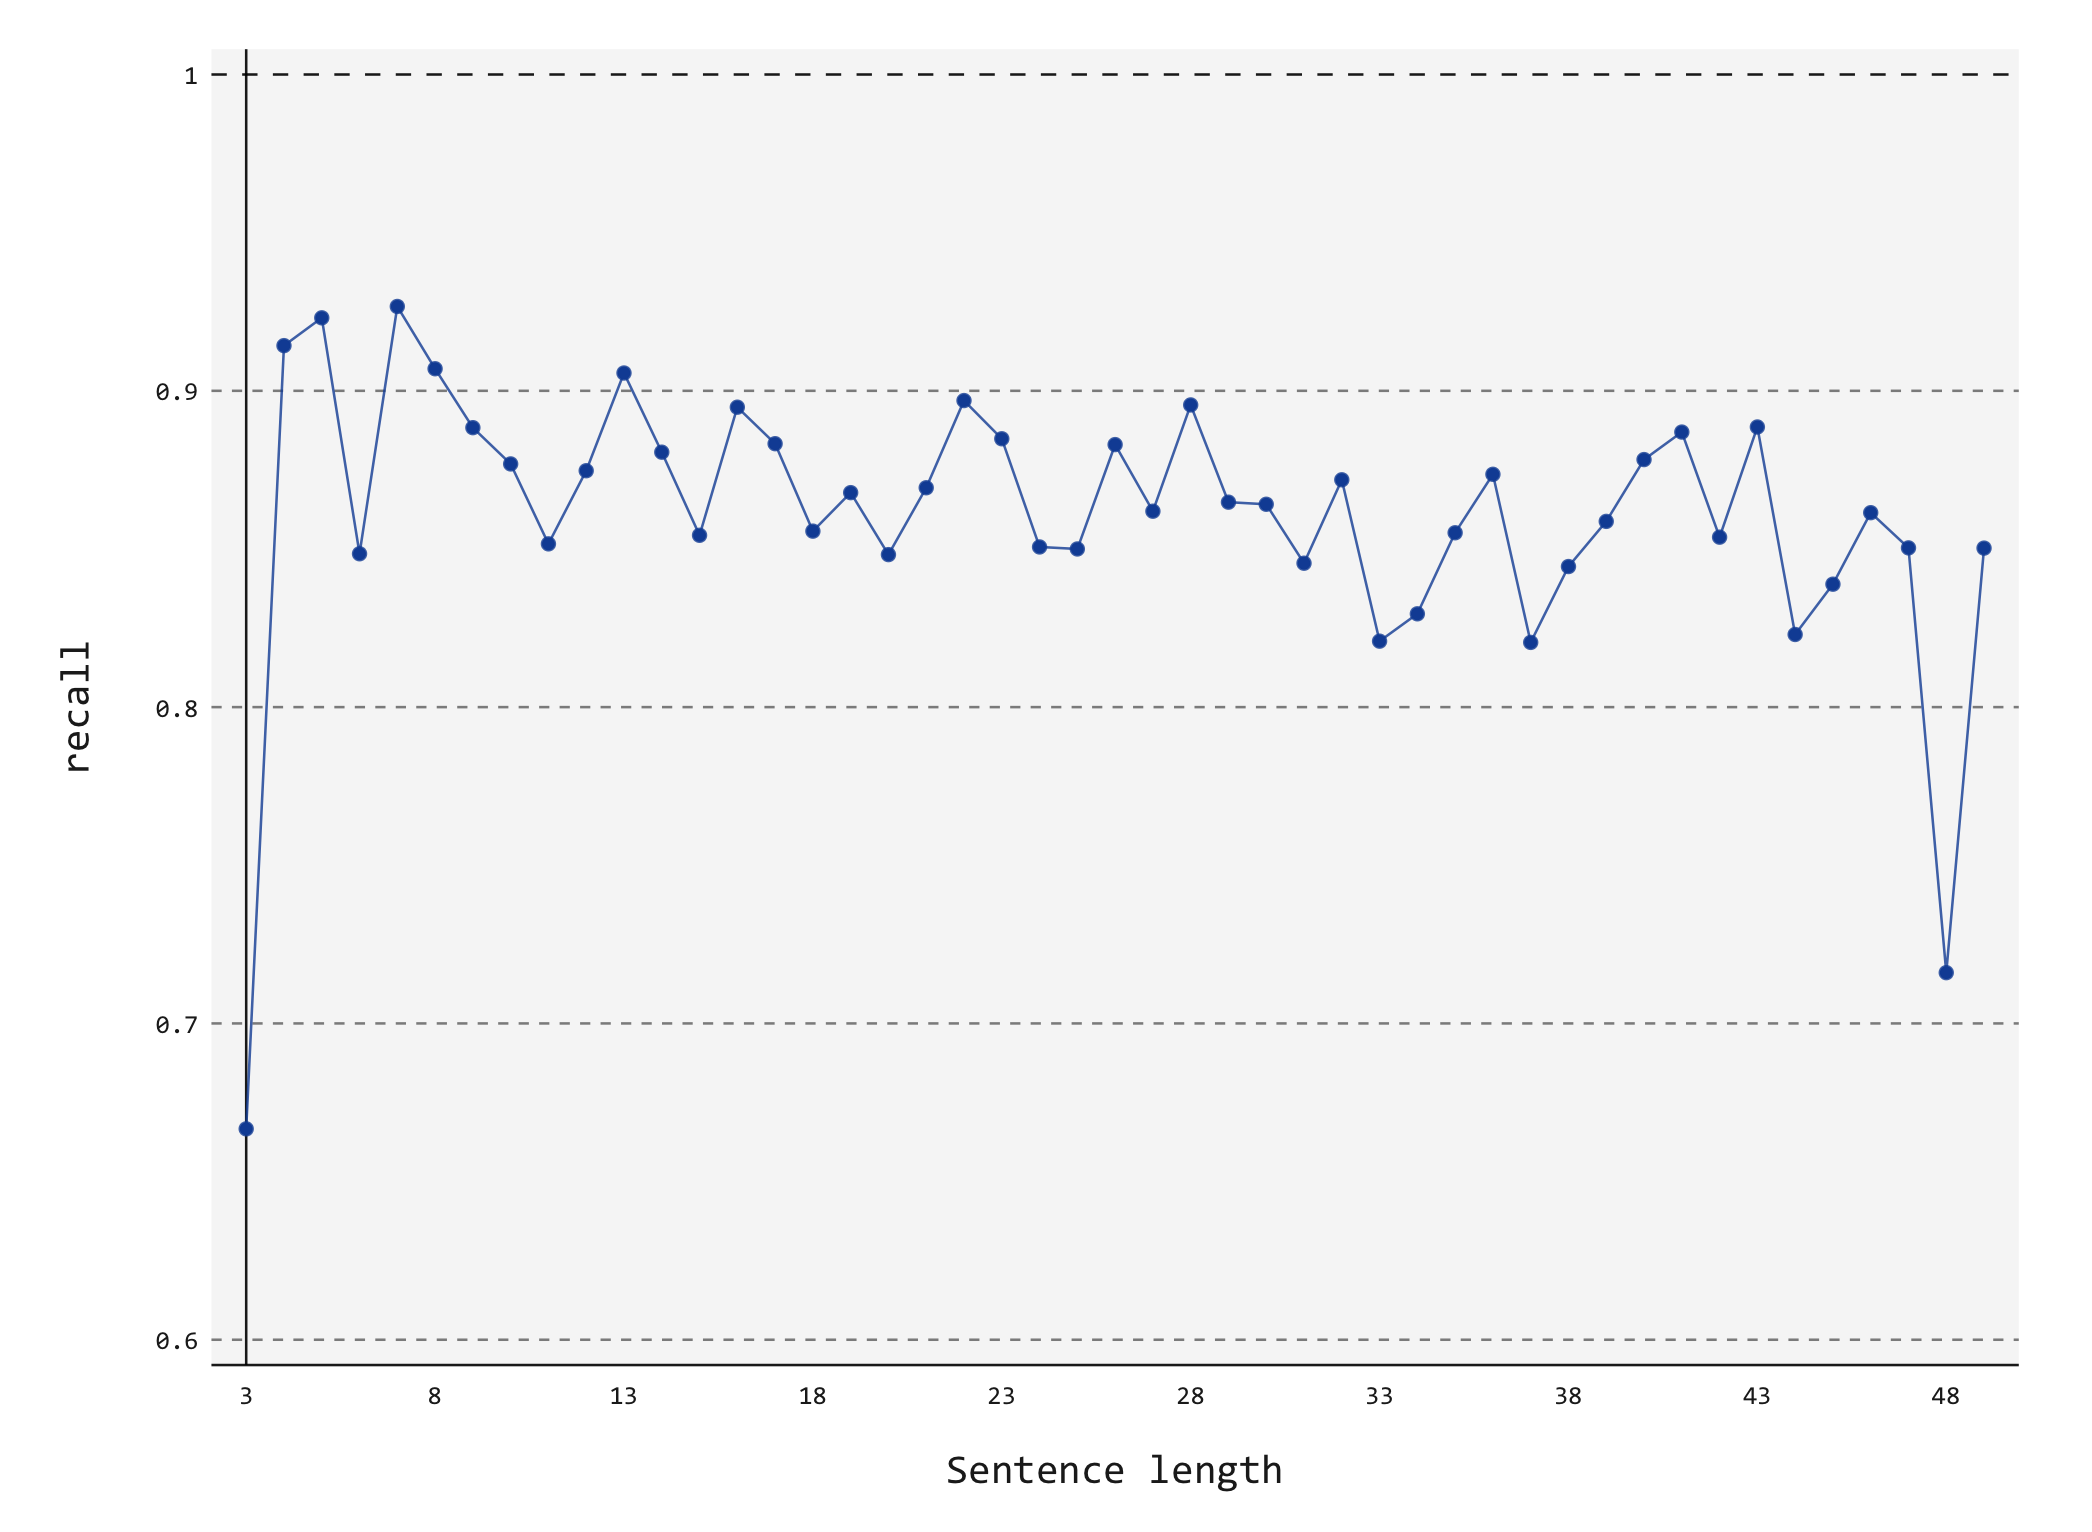
\includegraphics[width=\textwidth]{sentence_dm_lisbon_recall}
    \end{minipage}
    
    \begin{minipage}{0.50\textwidth}
        \centering
        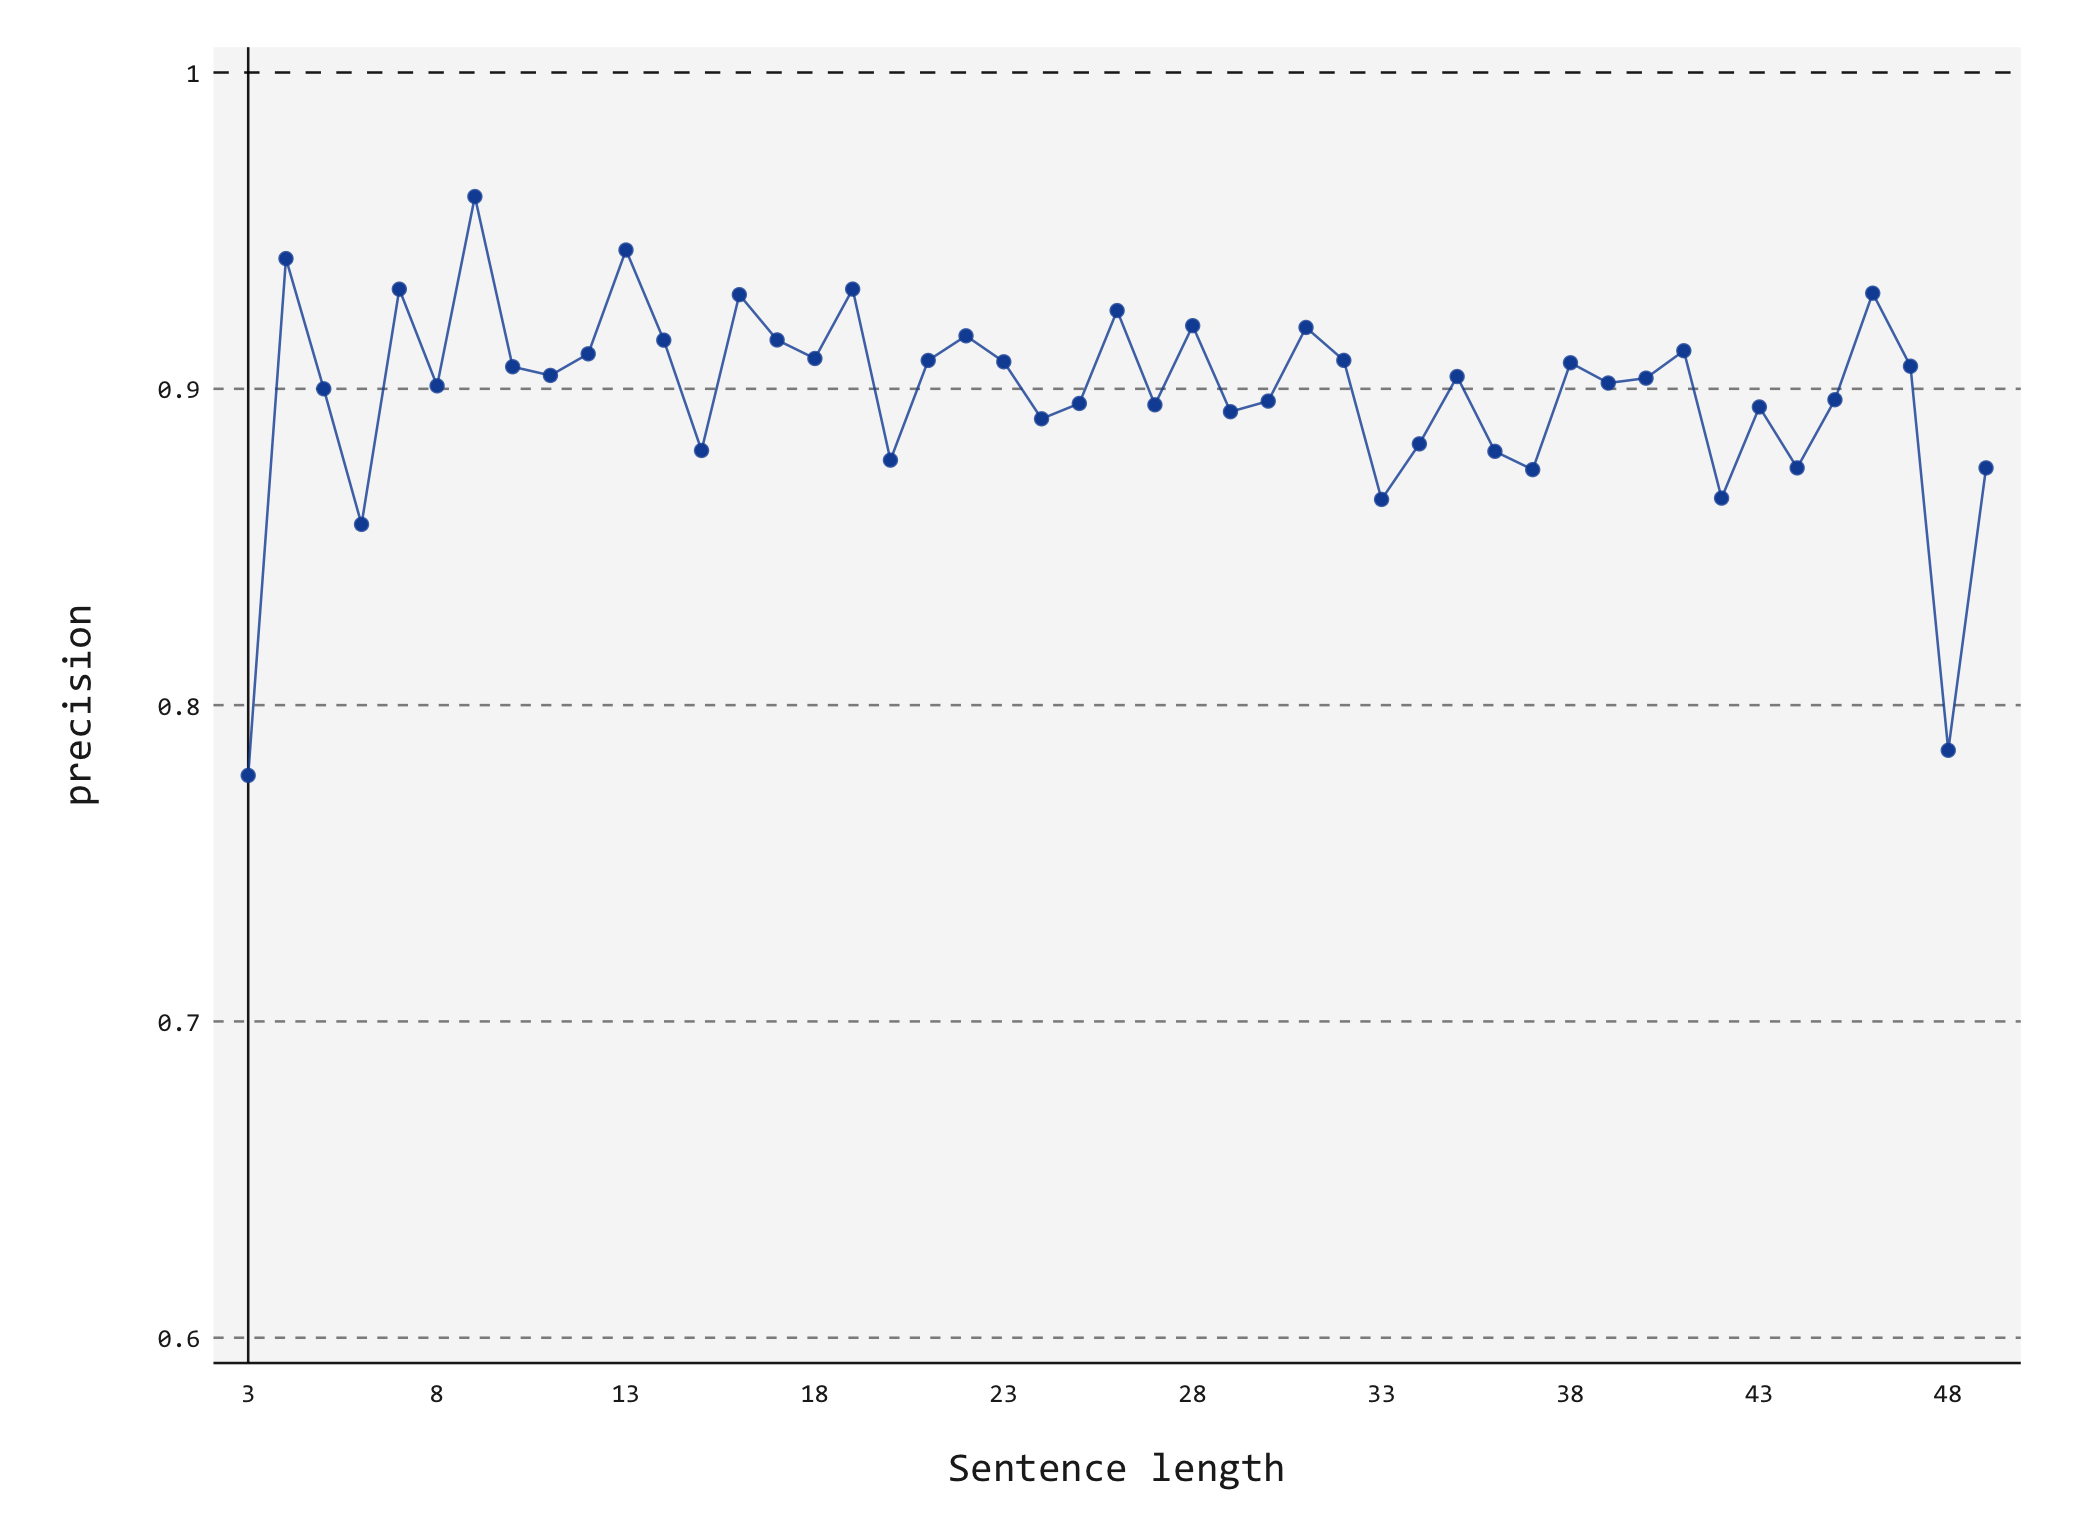
\includegraphics[width=\textwidth]{sentence_dm_peking_precision}
    \end{minipage}\hfill
    \begin{minipage}{0.50\textwidth}
        \centering
        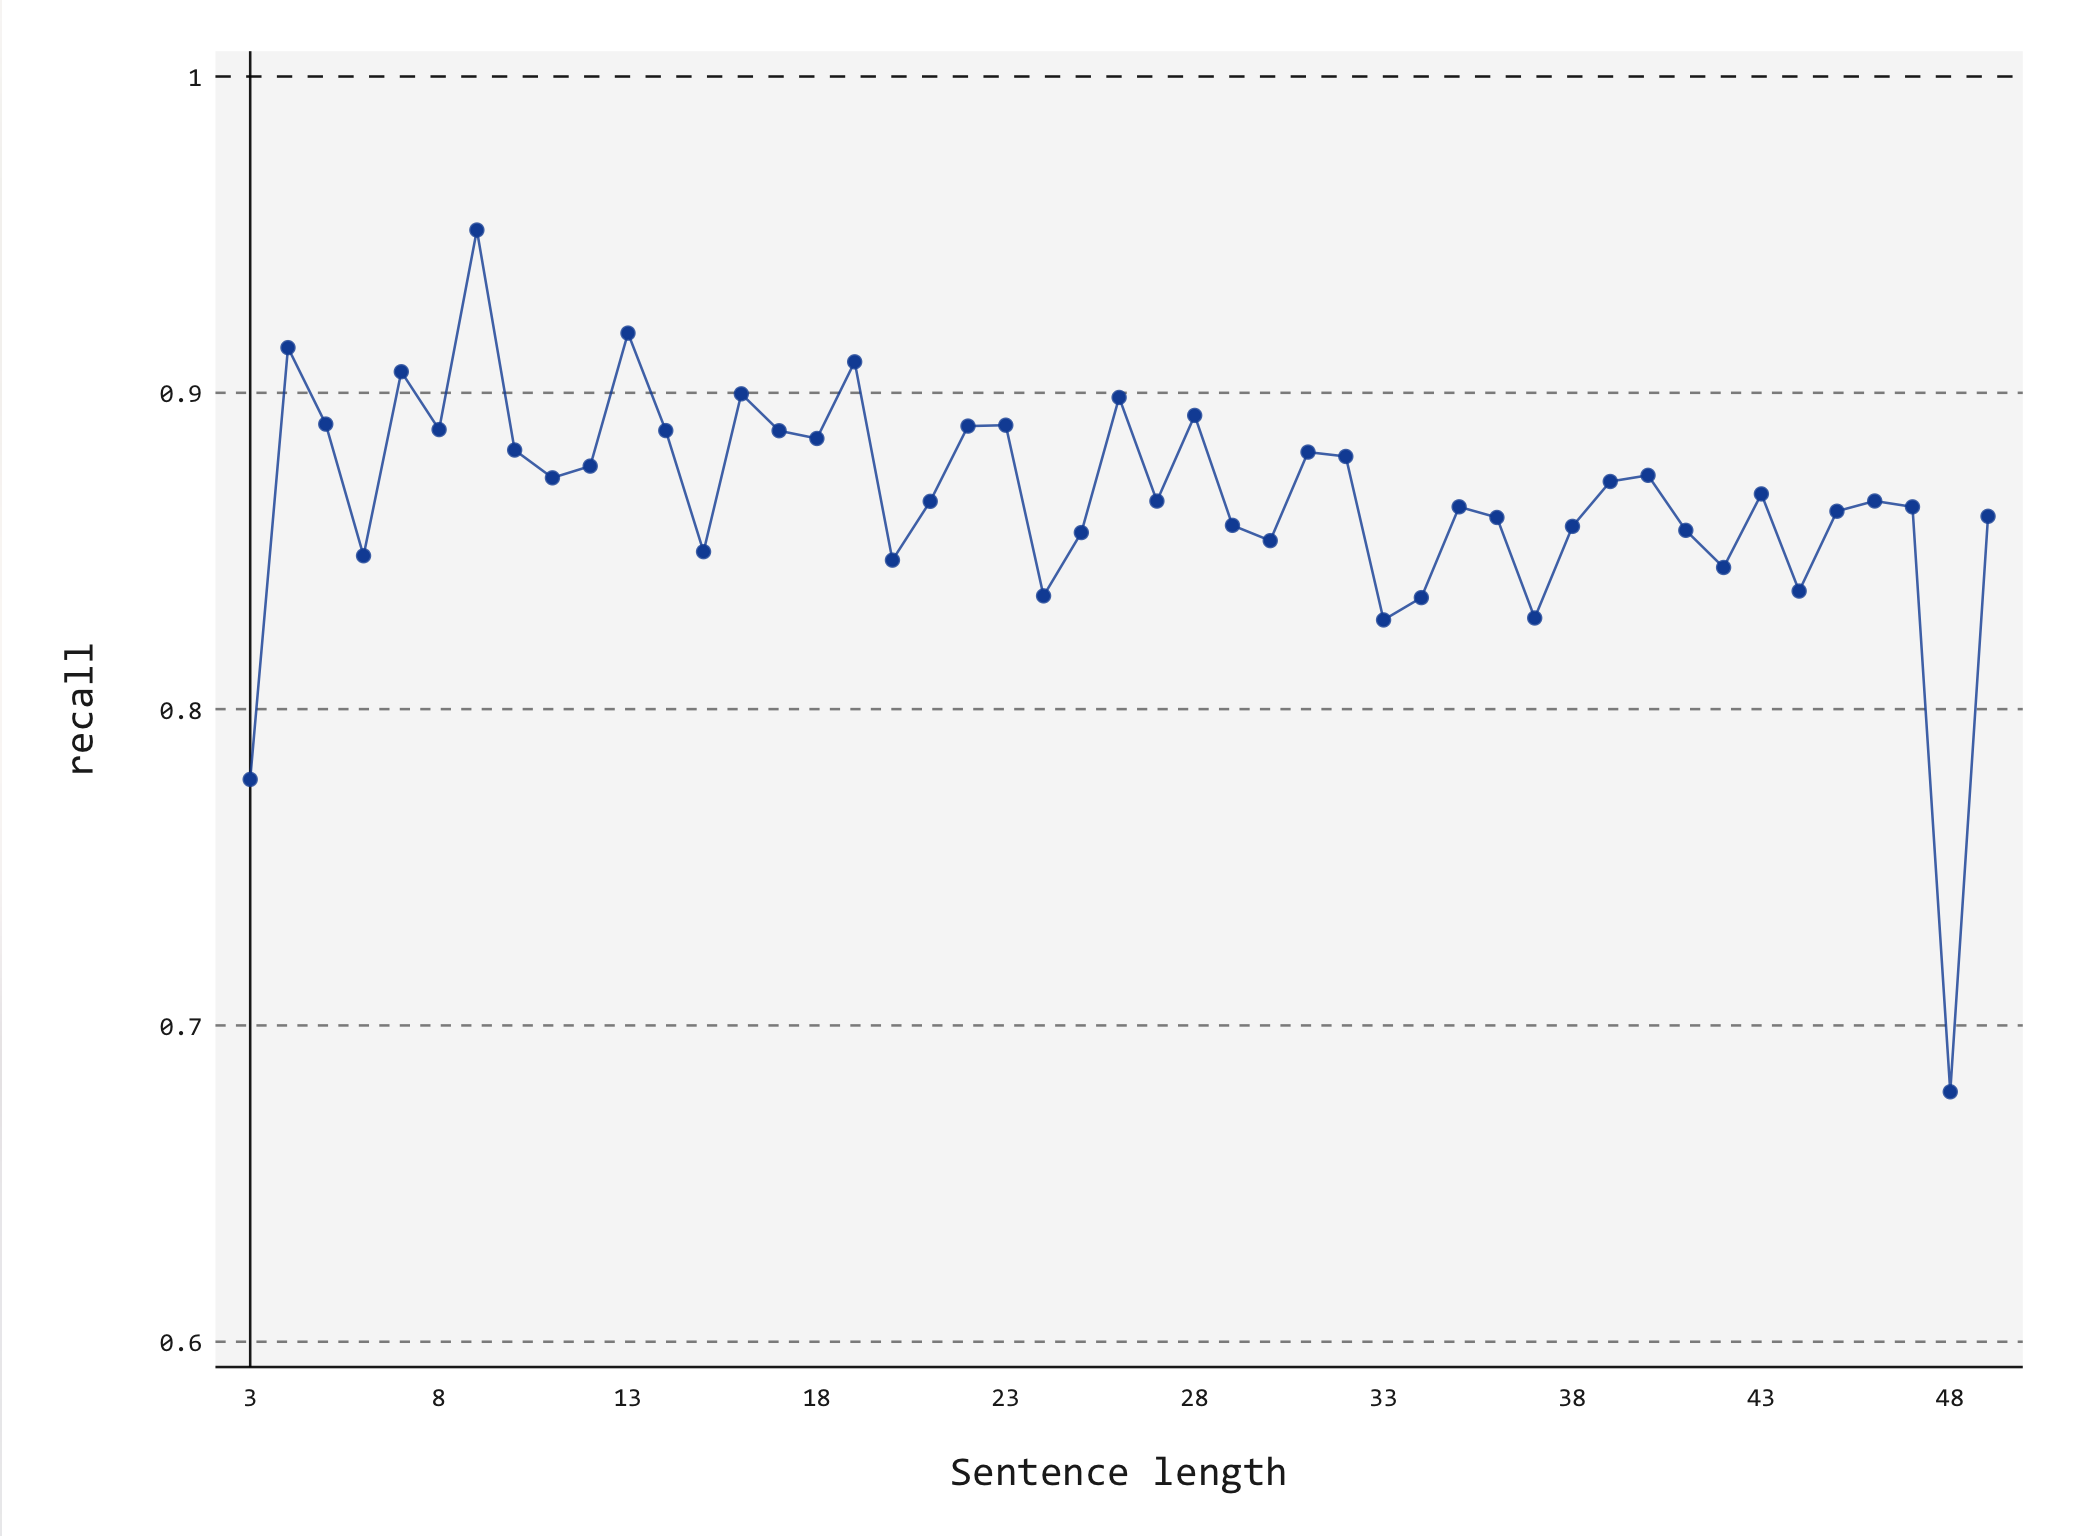
\includegraphics[width=\textwidth]{sentence_dm_peking_recall}
    \end{minipage}
    
    \begin{minipage}{0.50\textwidth}
        \centering
        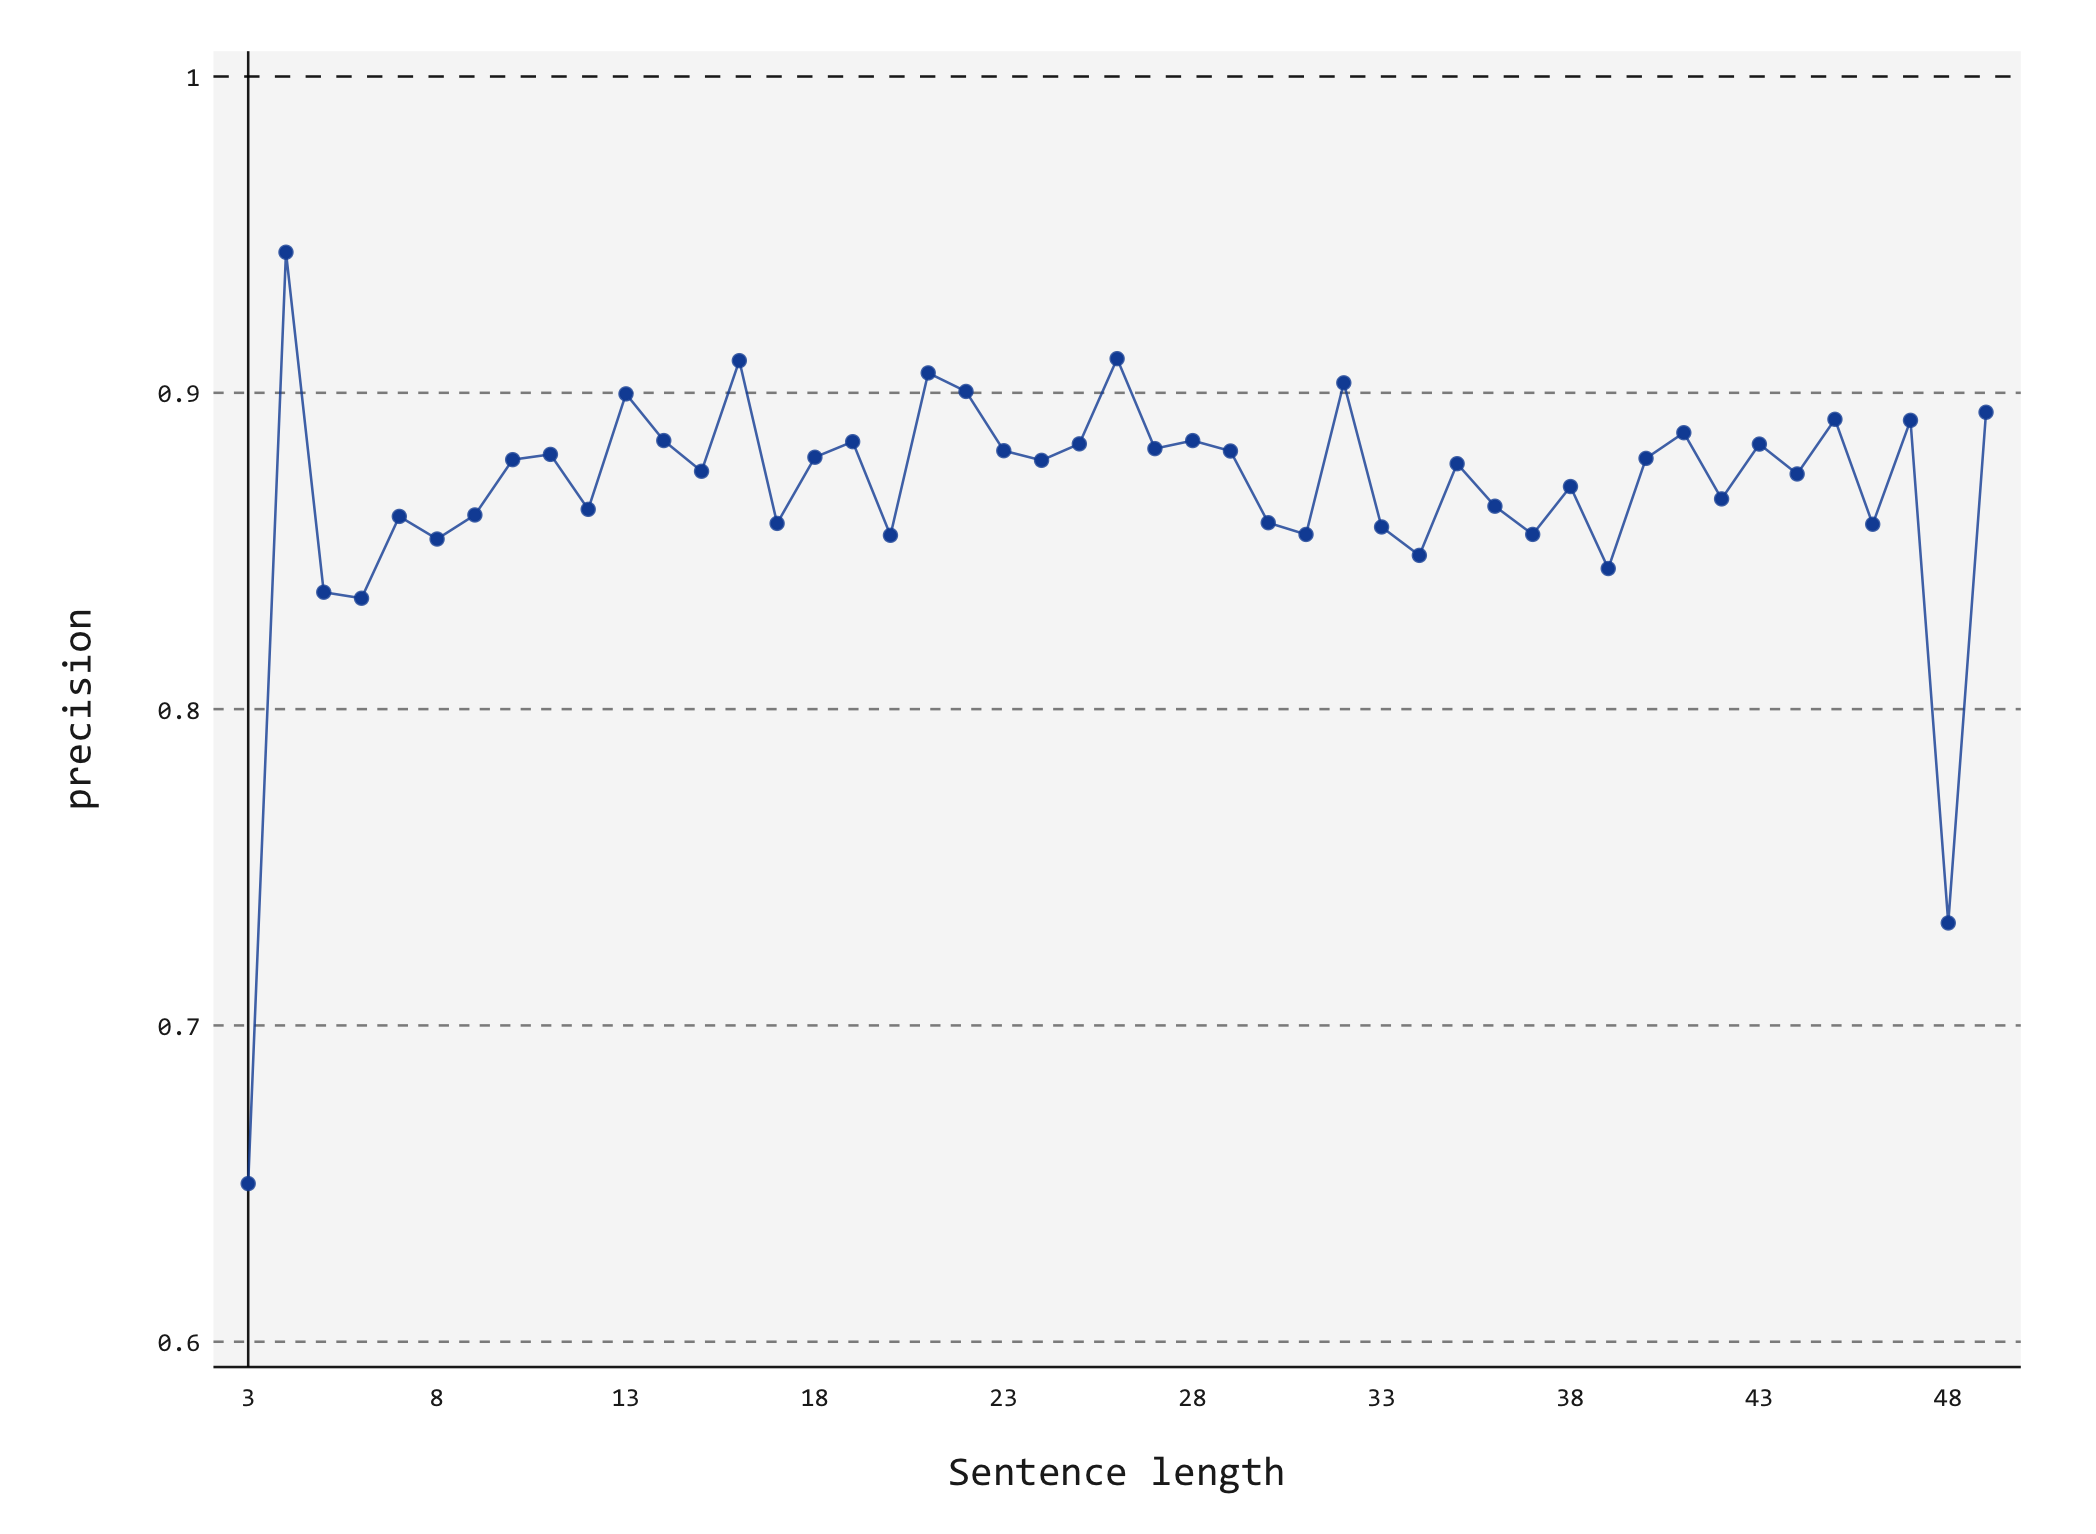
\includegraphics[width=\textwidth]{sentence_dm_turku_precision}
    \end{minipage}\hfill
    \begin{minipage}{0.50\textwidth}
        \centering
        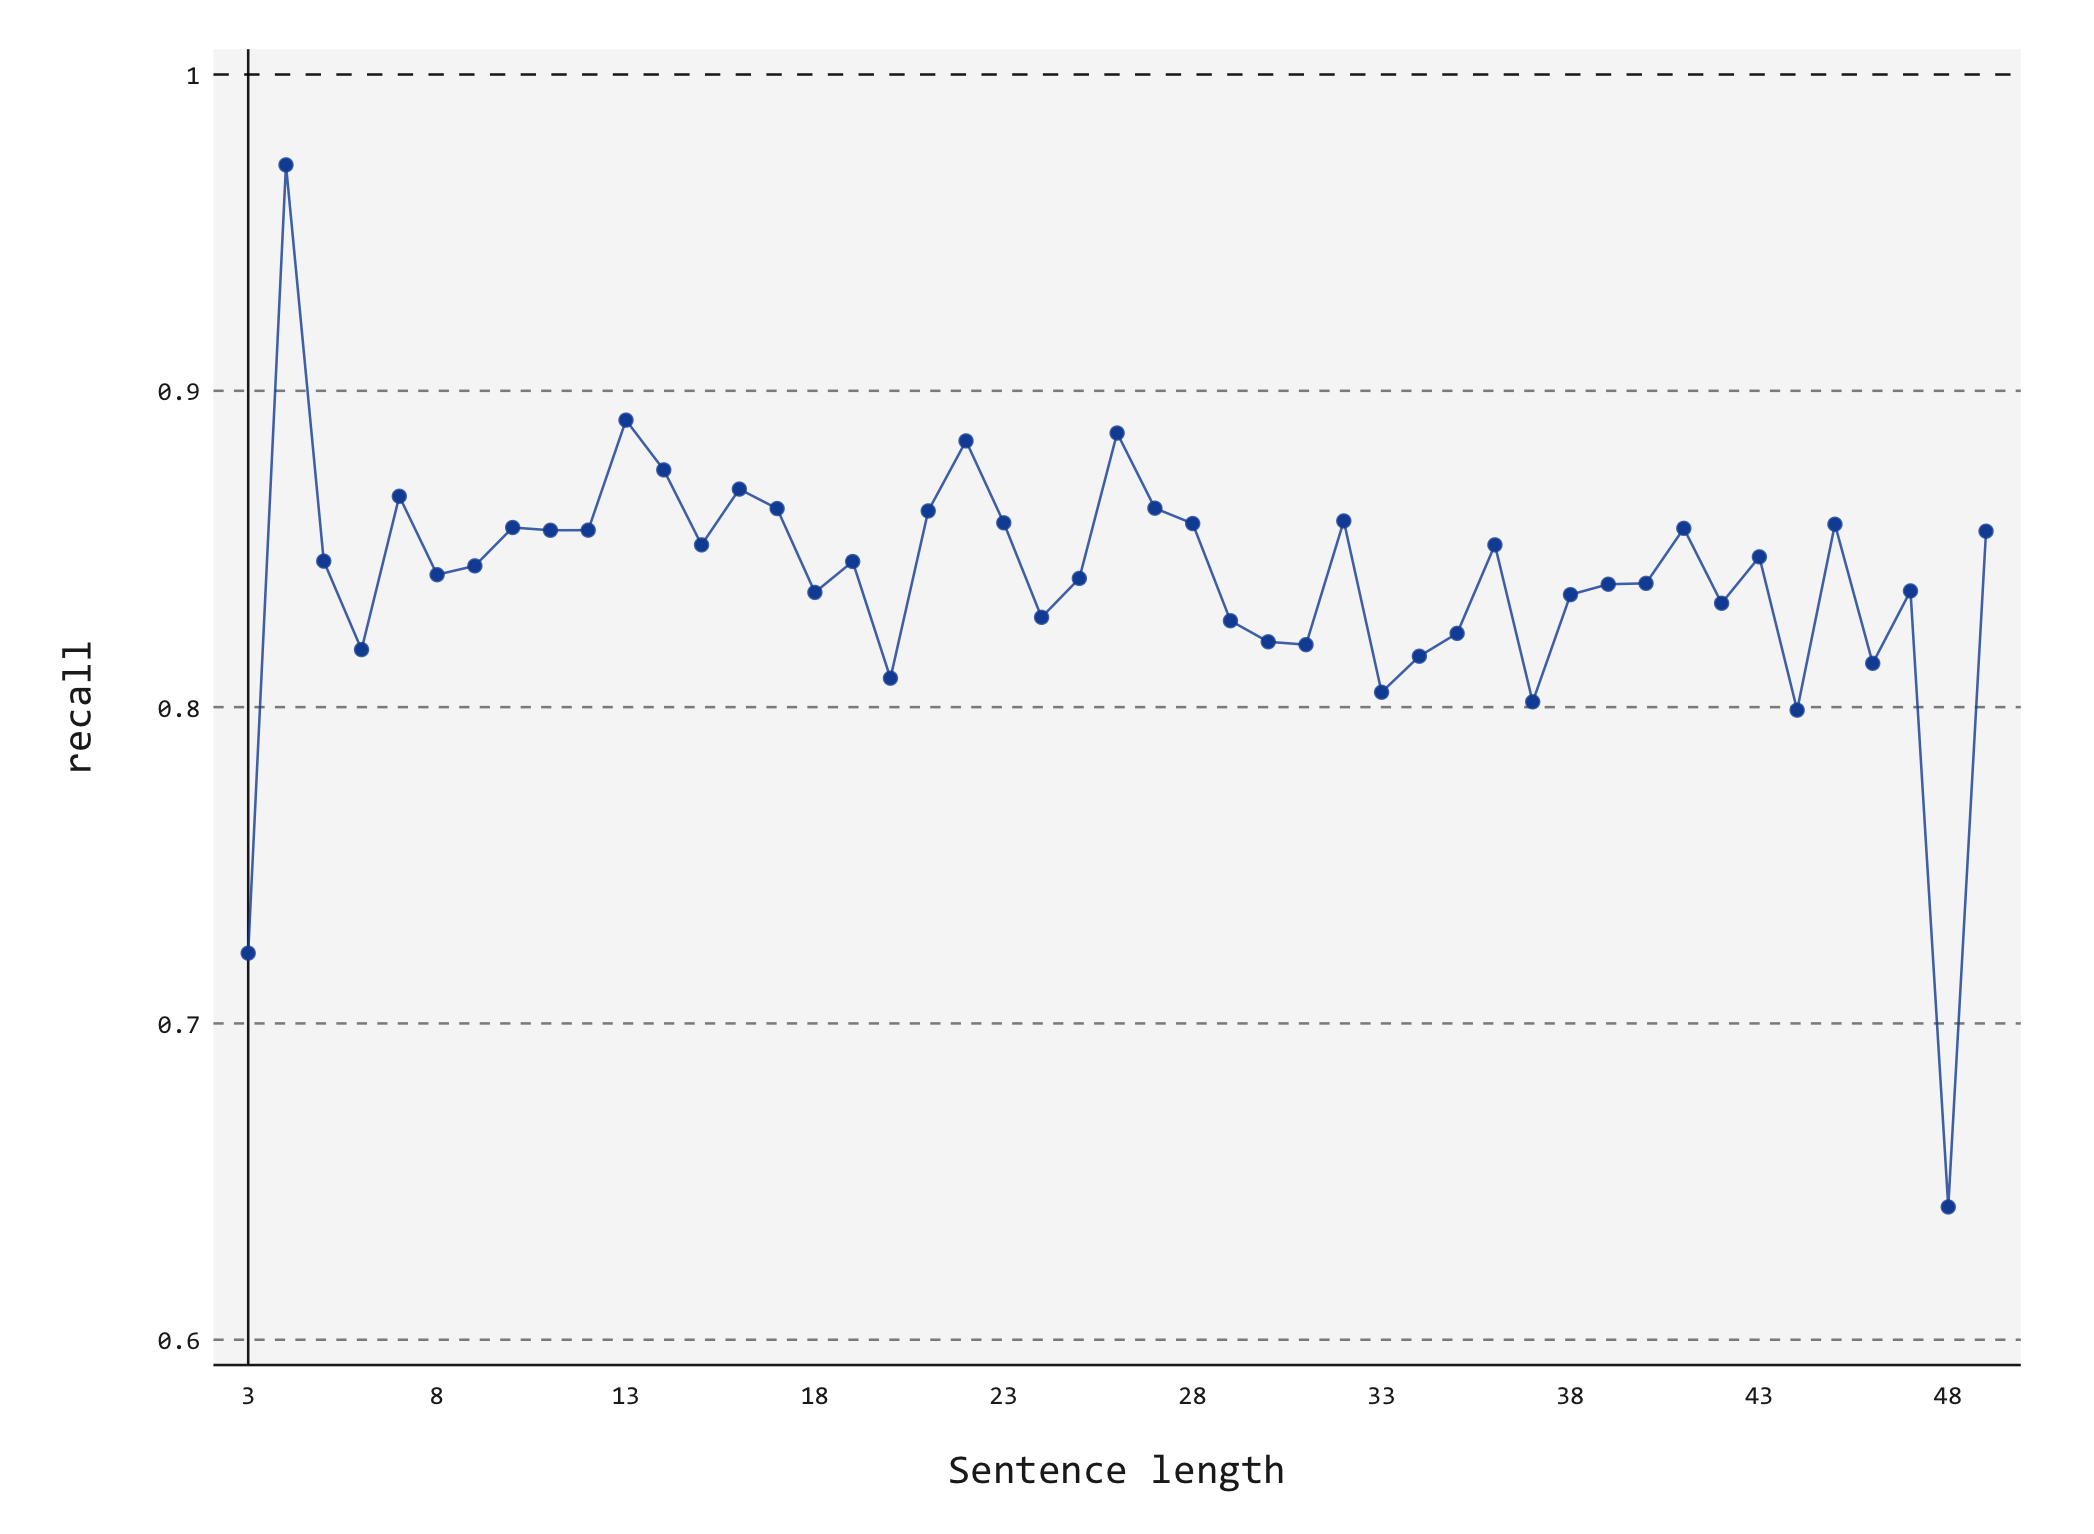
\includegraphics[width=\textwidth]{sentence_dm_turku_recall}
    \end{minipage}
    
    \caption{Labeled precision and recall of the Lisbon (top), Peking (middle), and Turku (bottom) parsing system on the DM target representation.}
    \label{fig:dm_s_length}
\end{figure}

\begin{figure}[h]
    \centering
    \begin{minipage}{0.50\textwidth}
        \centering
        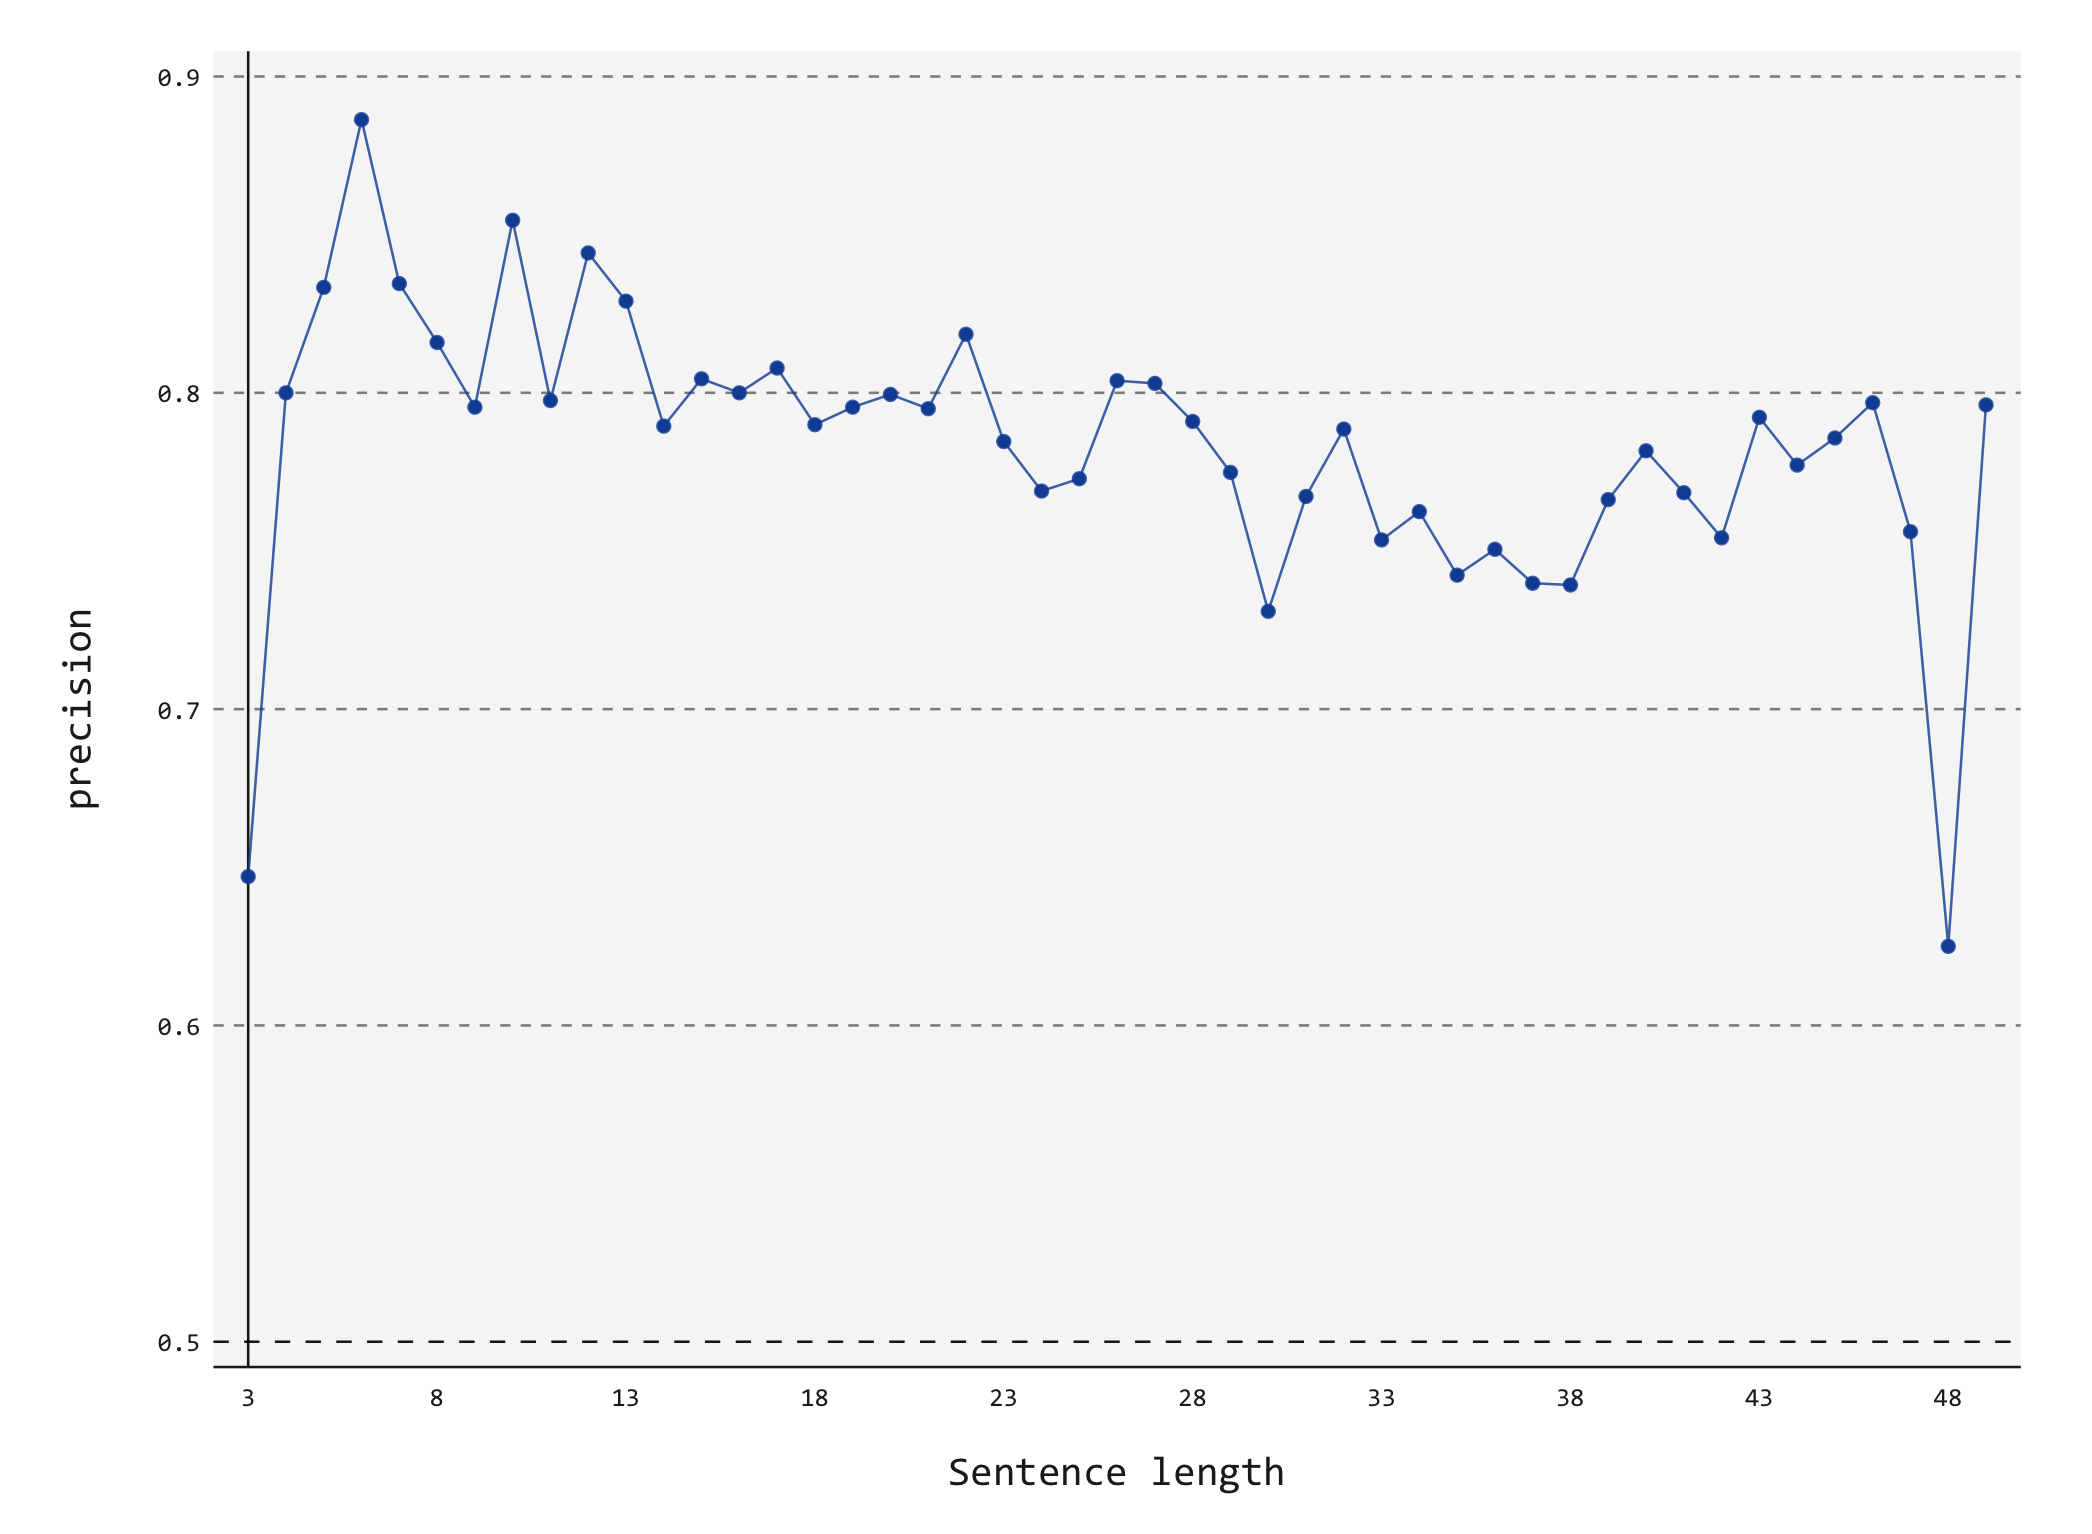
\includegraphics[width=\textwidth]{sentence_psd_lisbon_precision}
    \end{minipage}\hfill
    \begin{minipage}{0.50\textwidth}
        \centering
        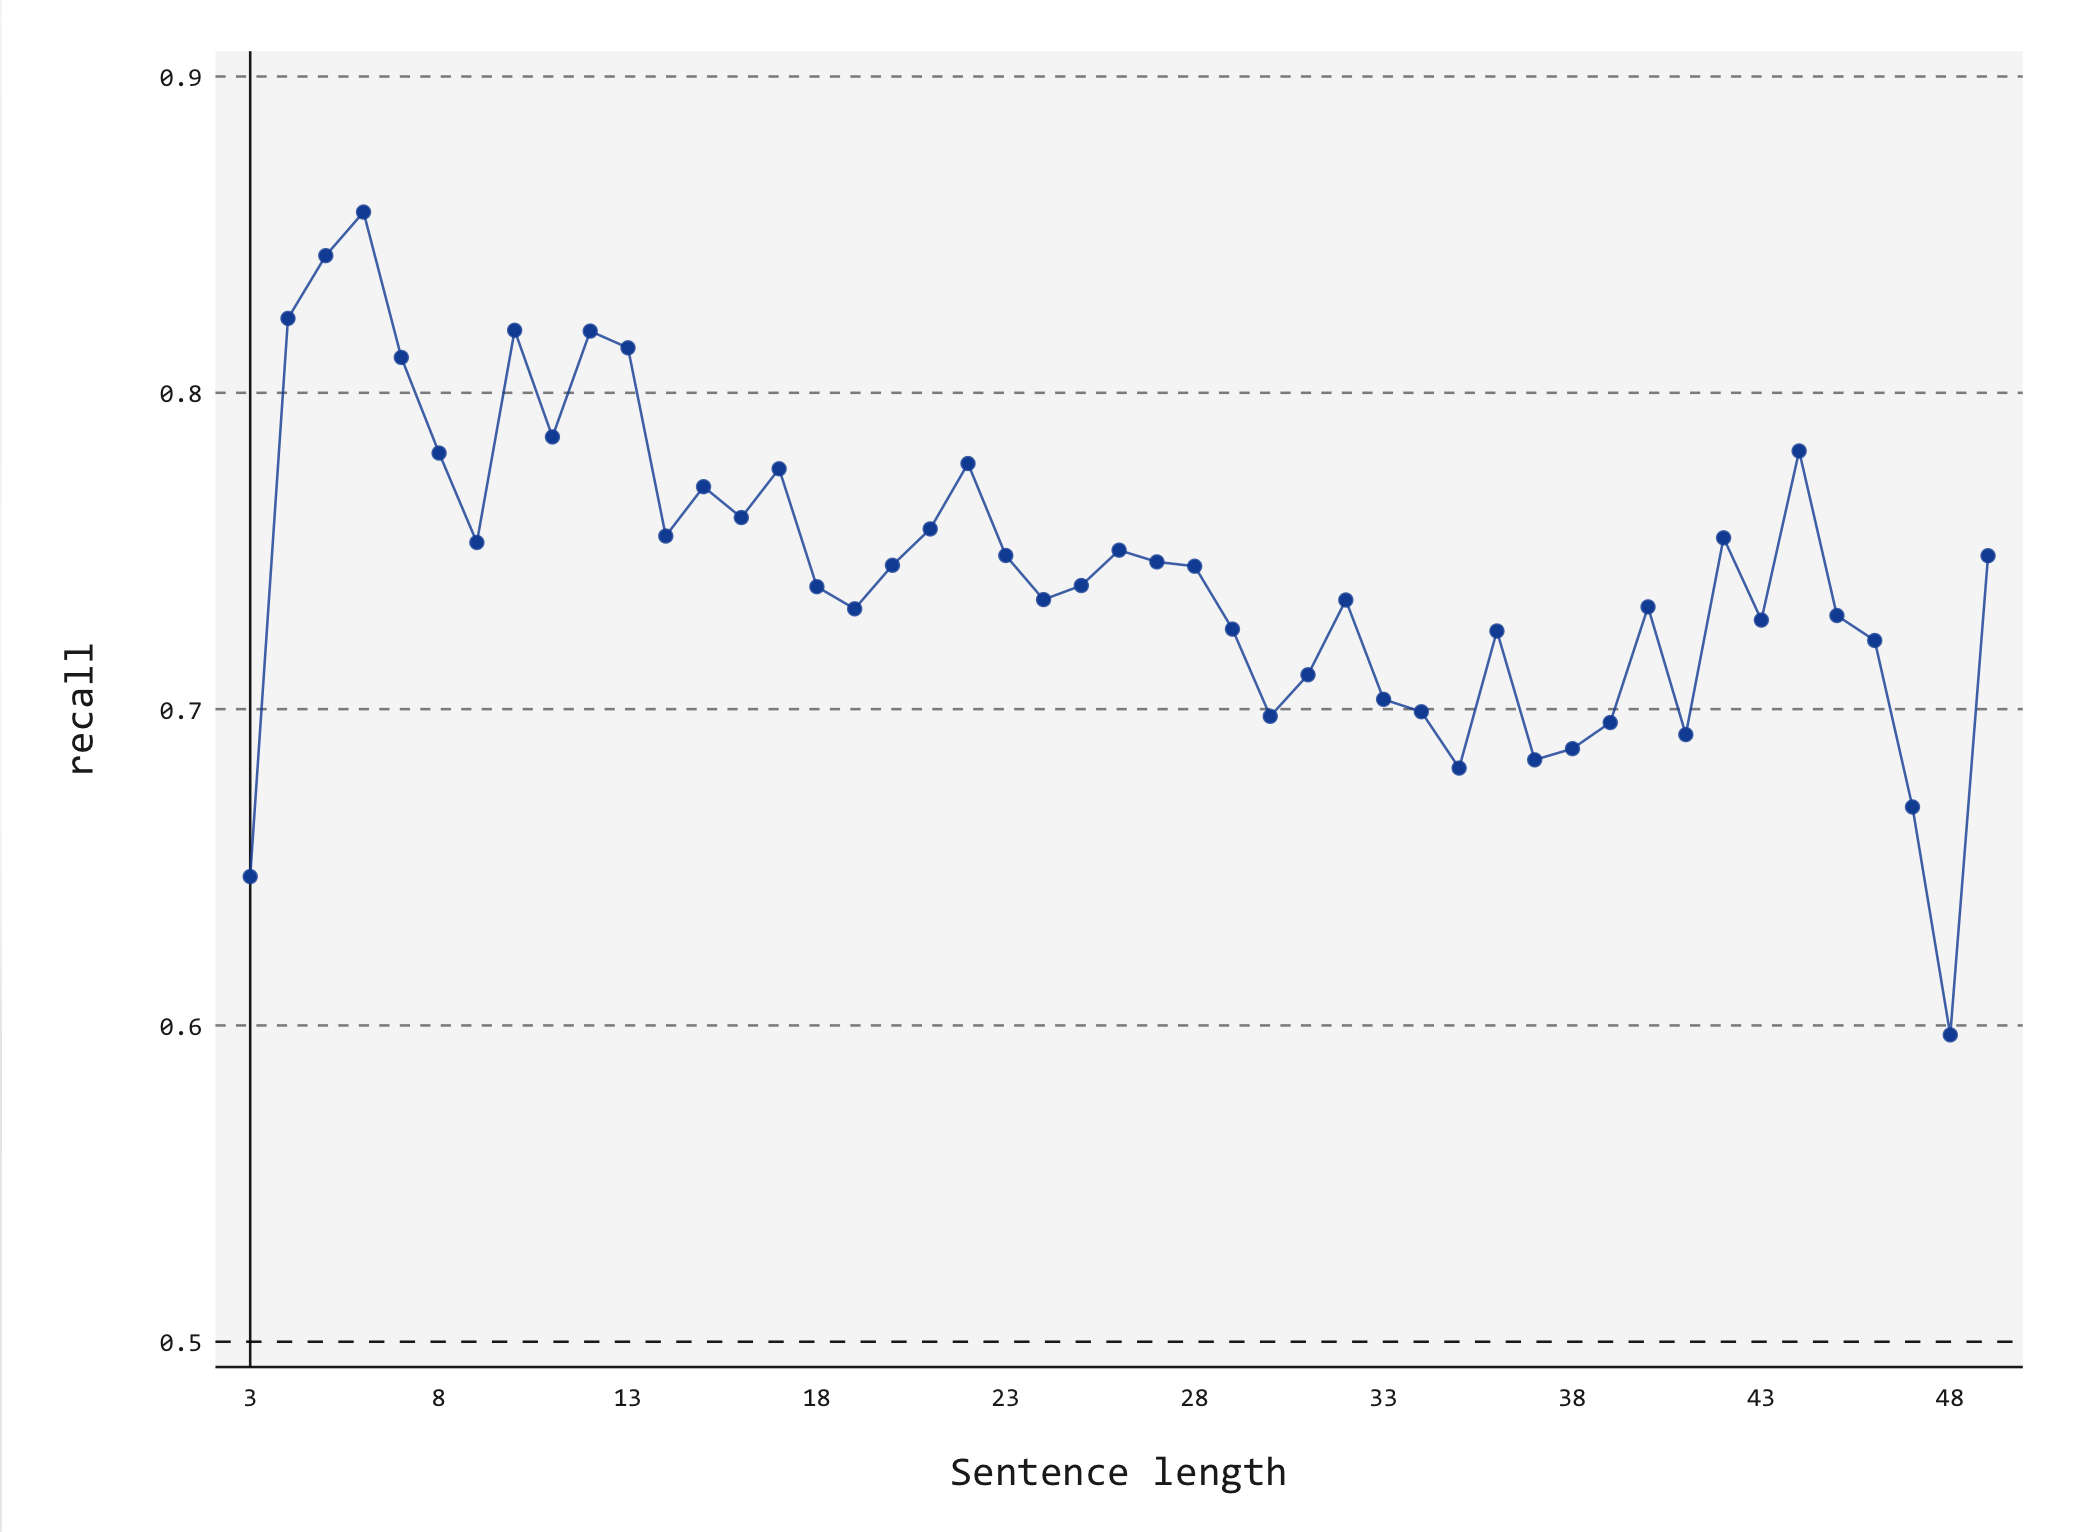
\includegraphics[width=\textwidth]{sentence_psd_lisbon_recall}
    \end{minipage}
    
    \begin{minipage}{0.50\textwidth}
        \centering
        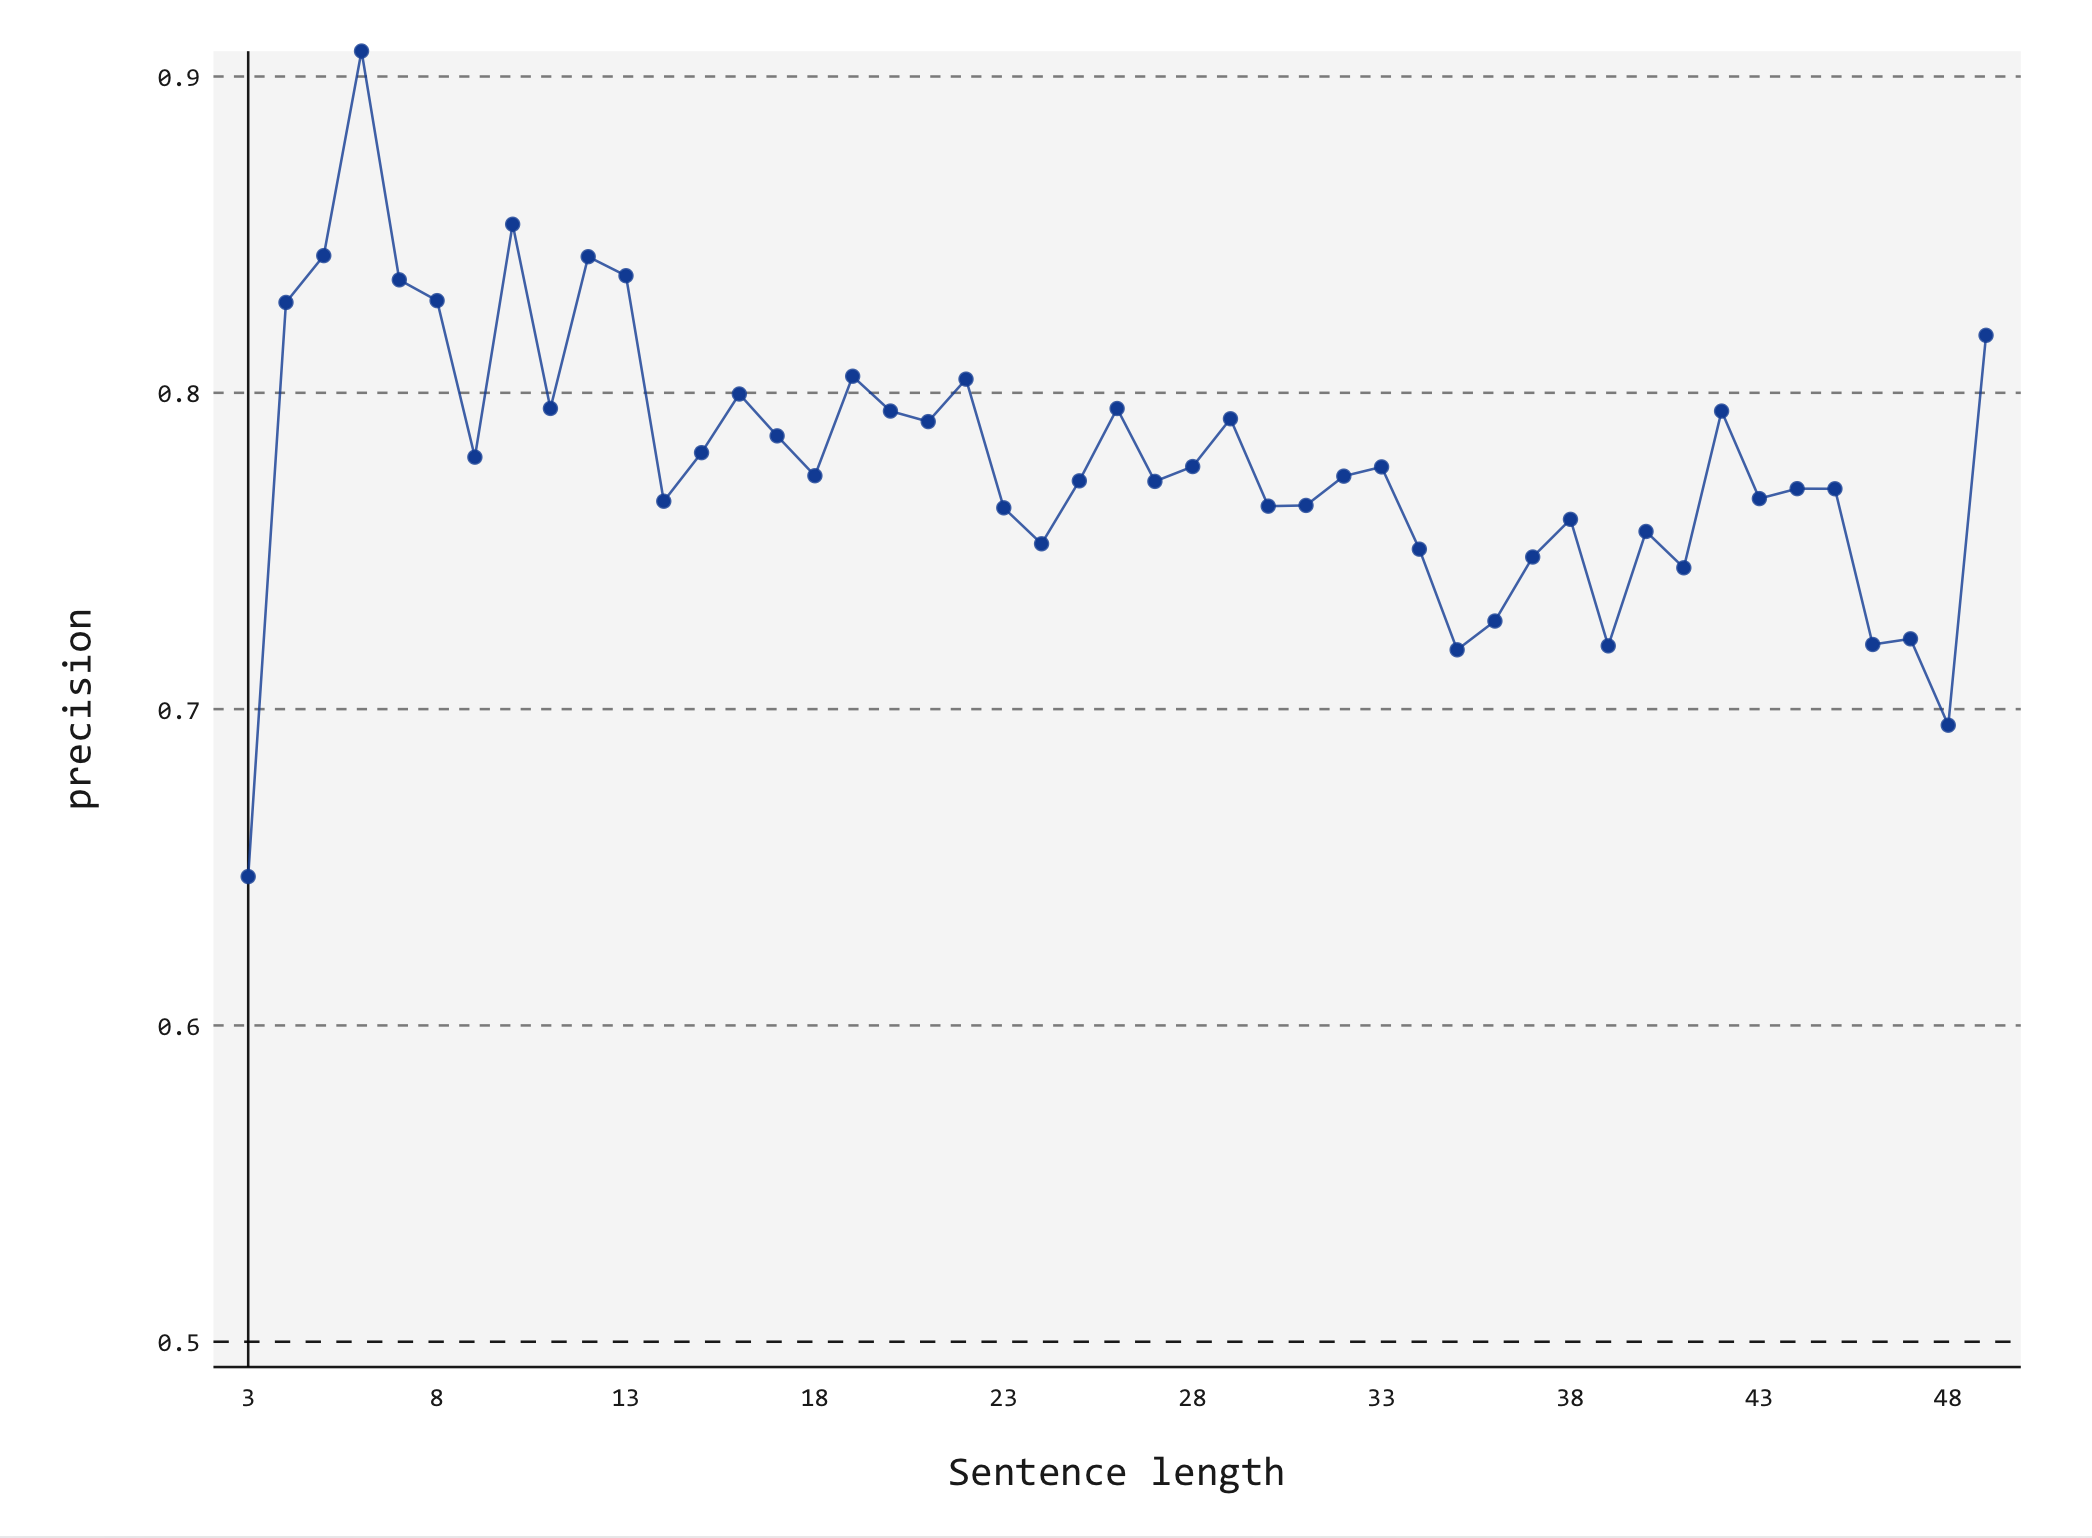
\includegraphics[width=\textwidth]{sentence_psd_peking_precision}
    \end{minipage}\hfill
    \begin{minipage}{0.50\textwidth}
        \centering
        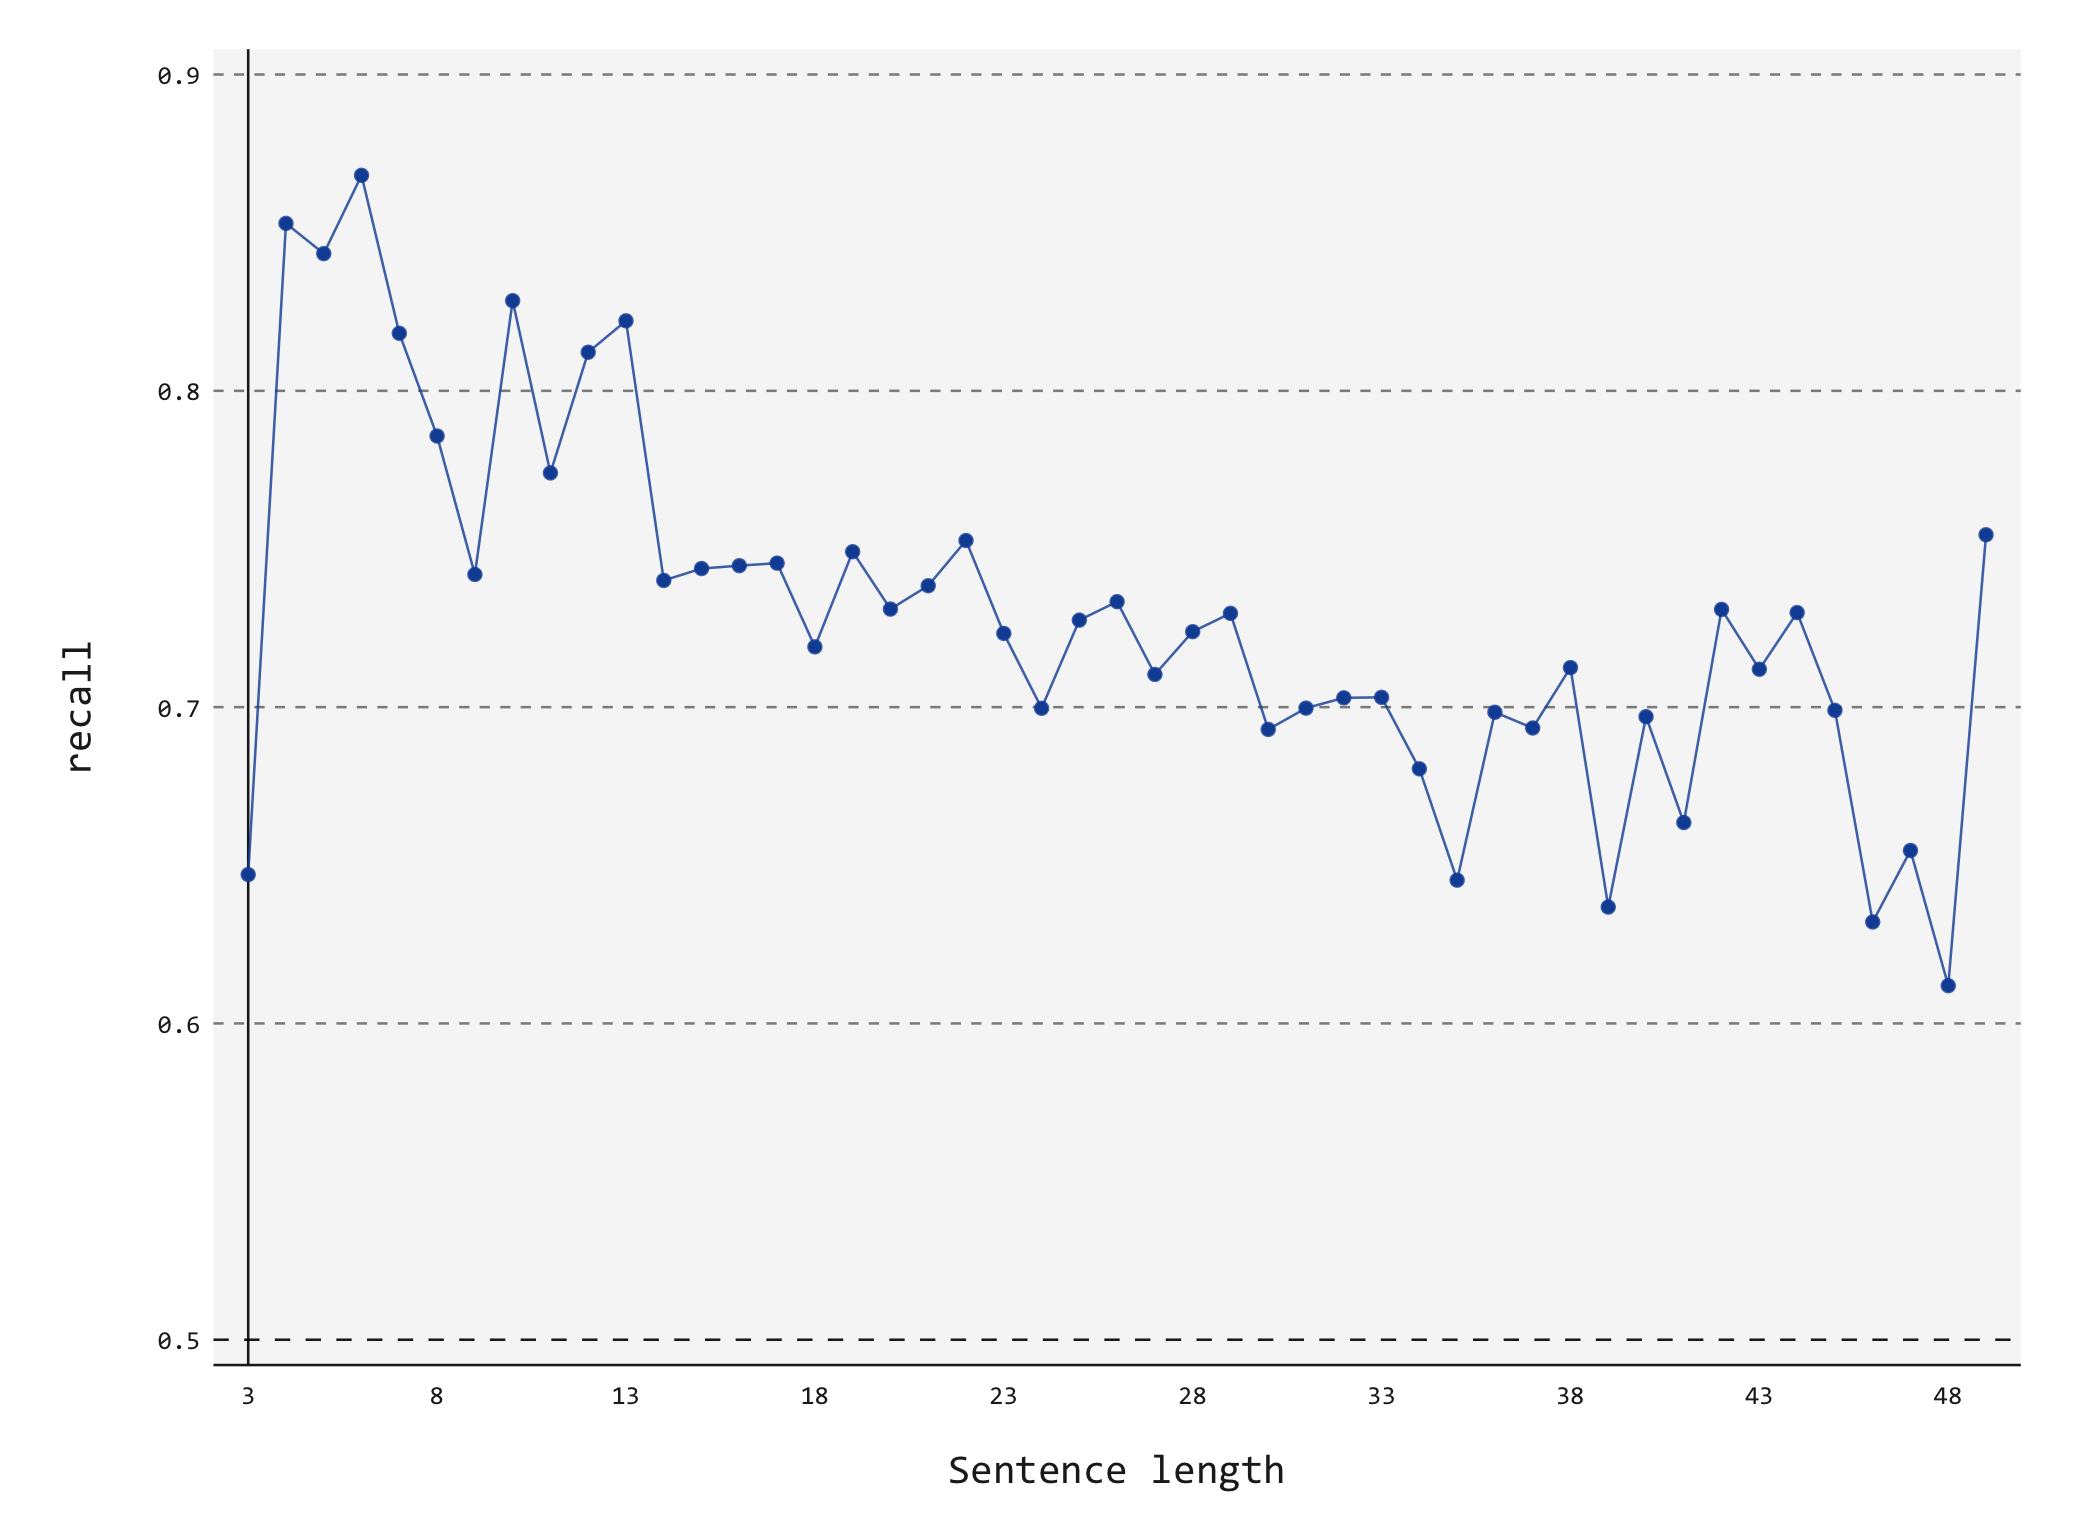
\includegraphics[width=\textwidth]{sentence_psd_peking_recall}
    \end{minipage}
    
    \begin{minipage}{0.50\textwidth}
        \centering
        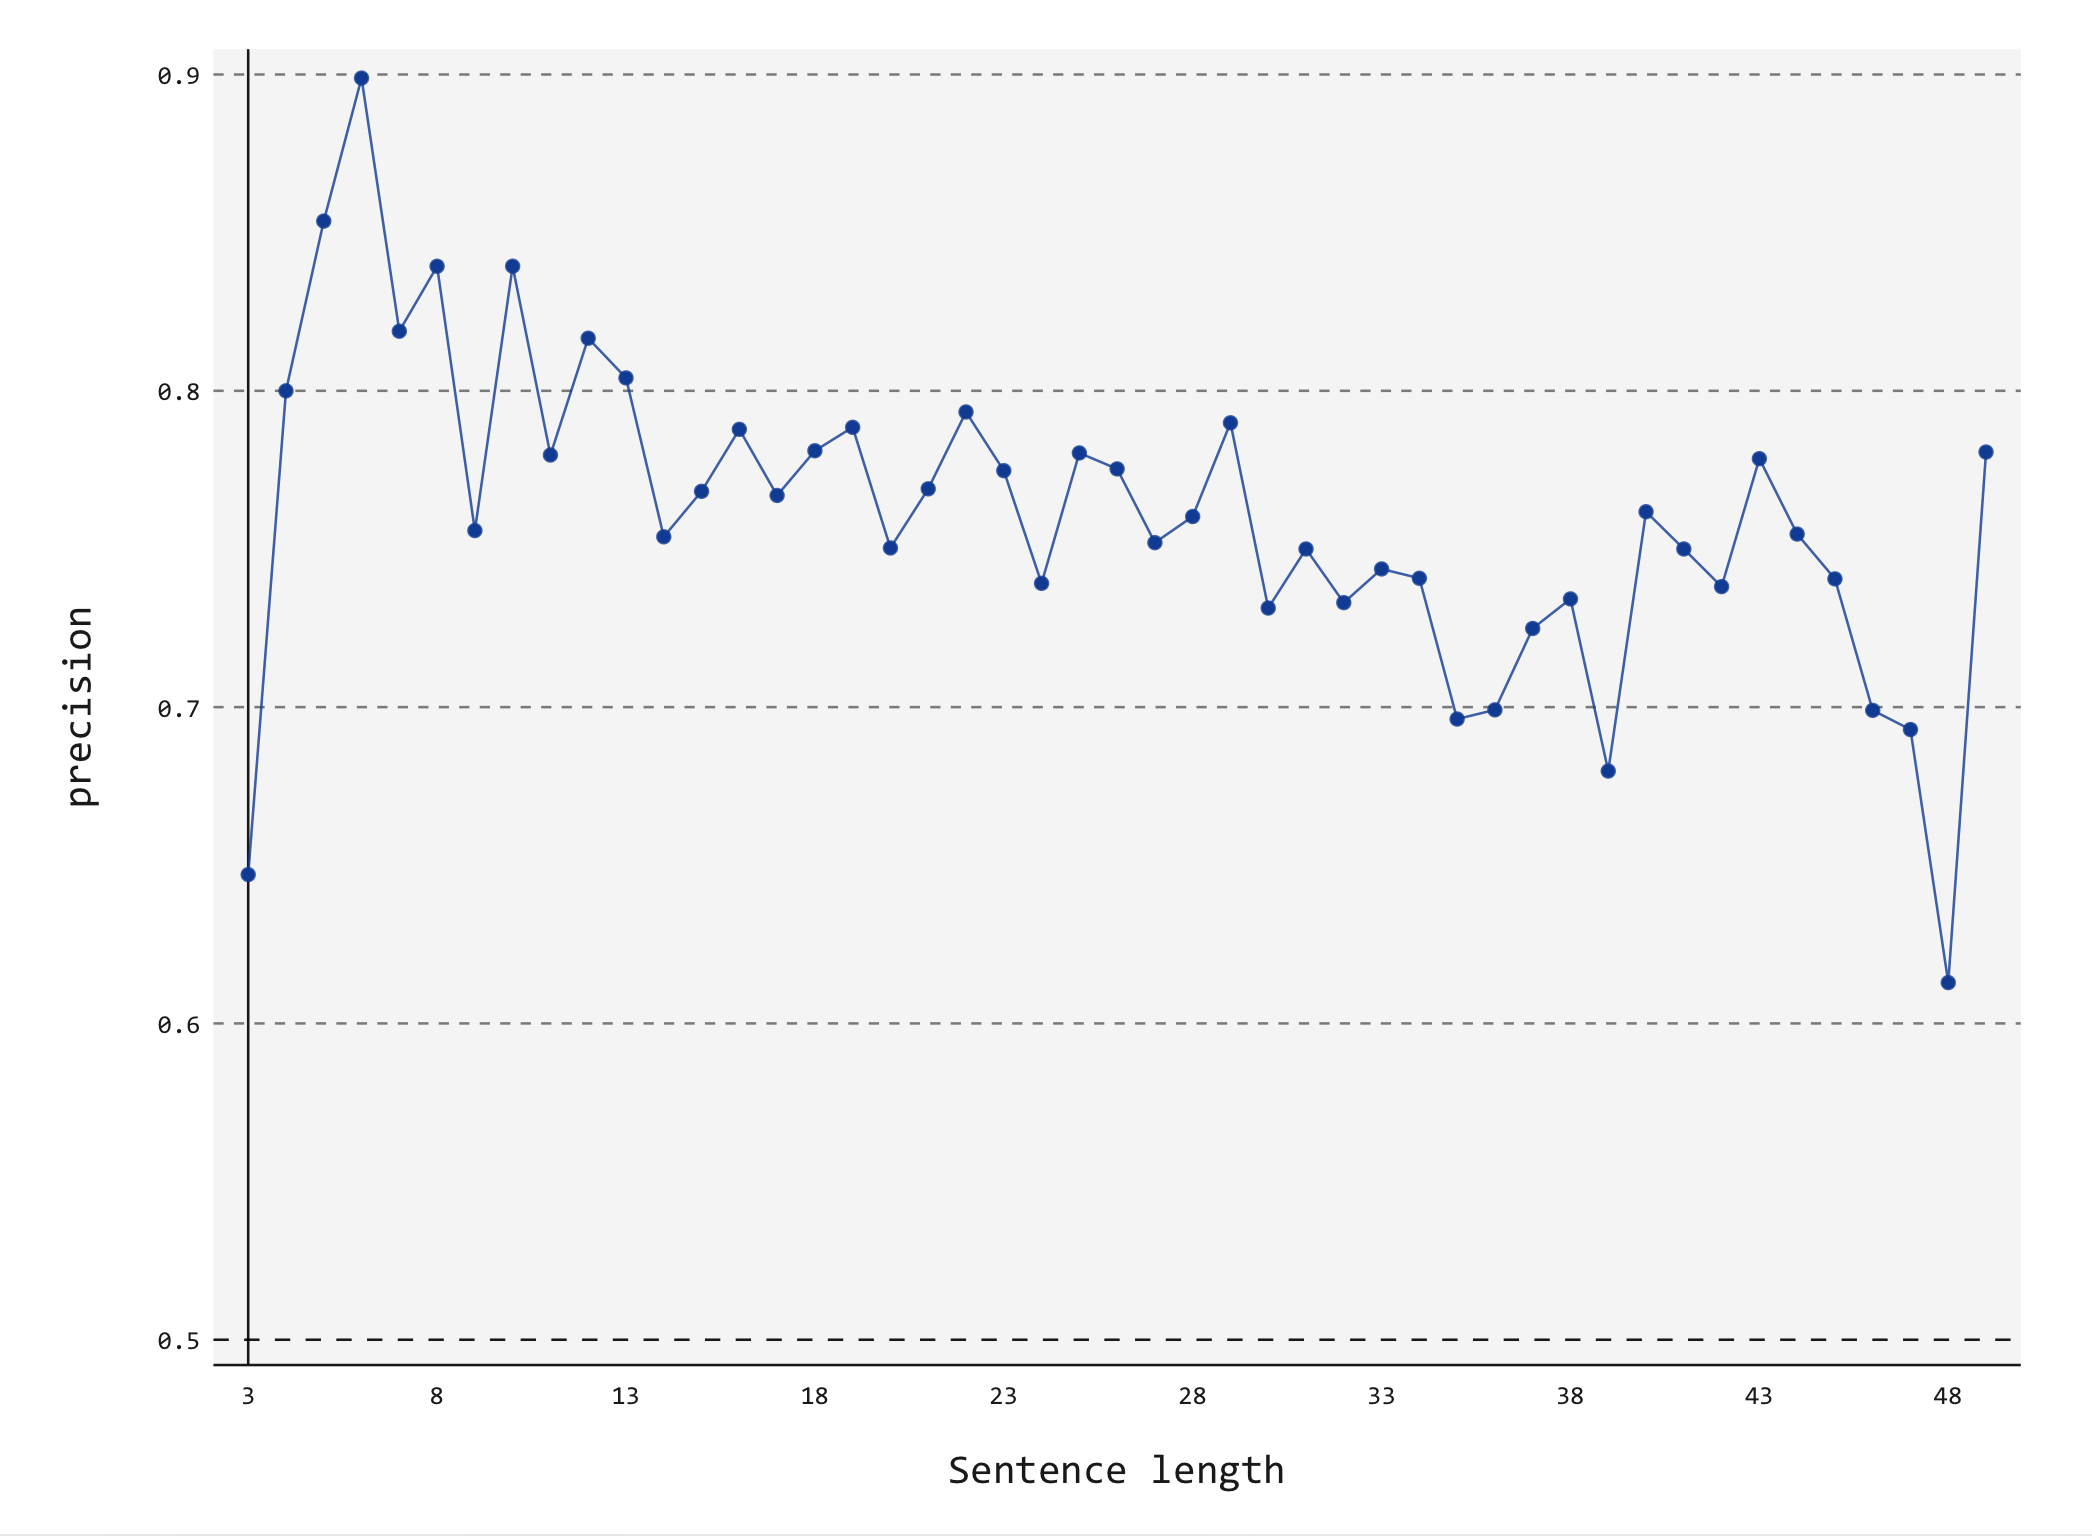
\includegraphics[width=\textwidth]{sentence_psd_turku_precision}
    \end{minipage}\hfill
    \begin{minipage}{0.50\textwidth}
        \centering
        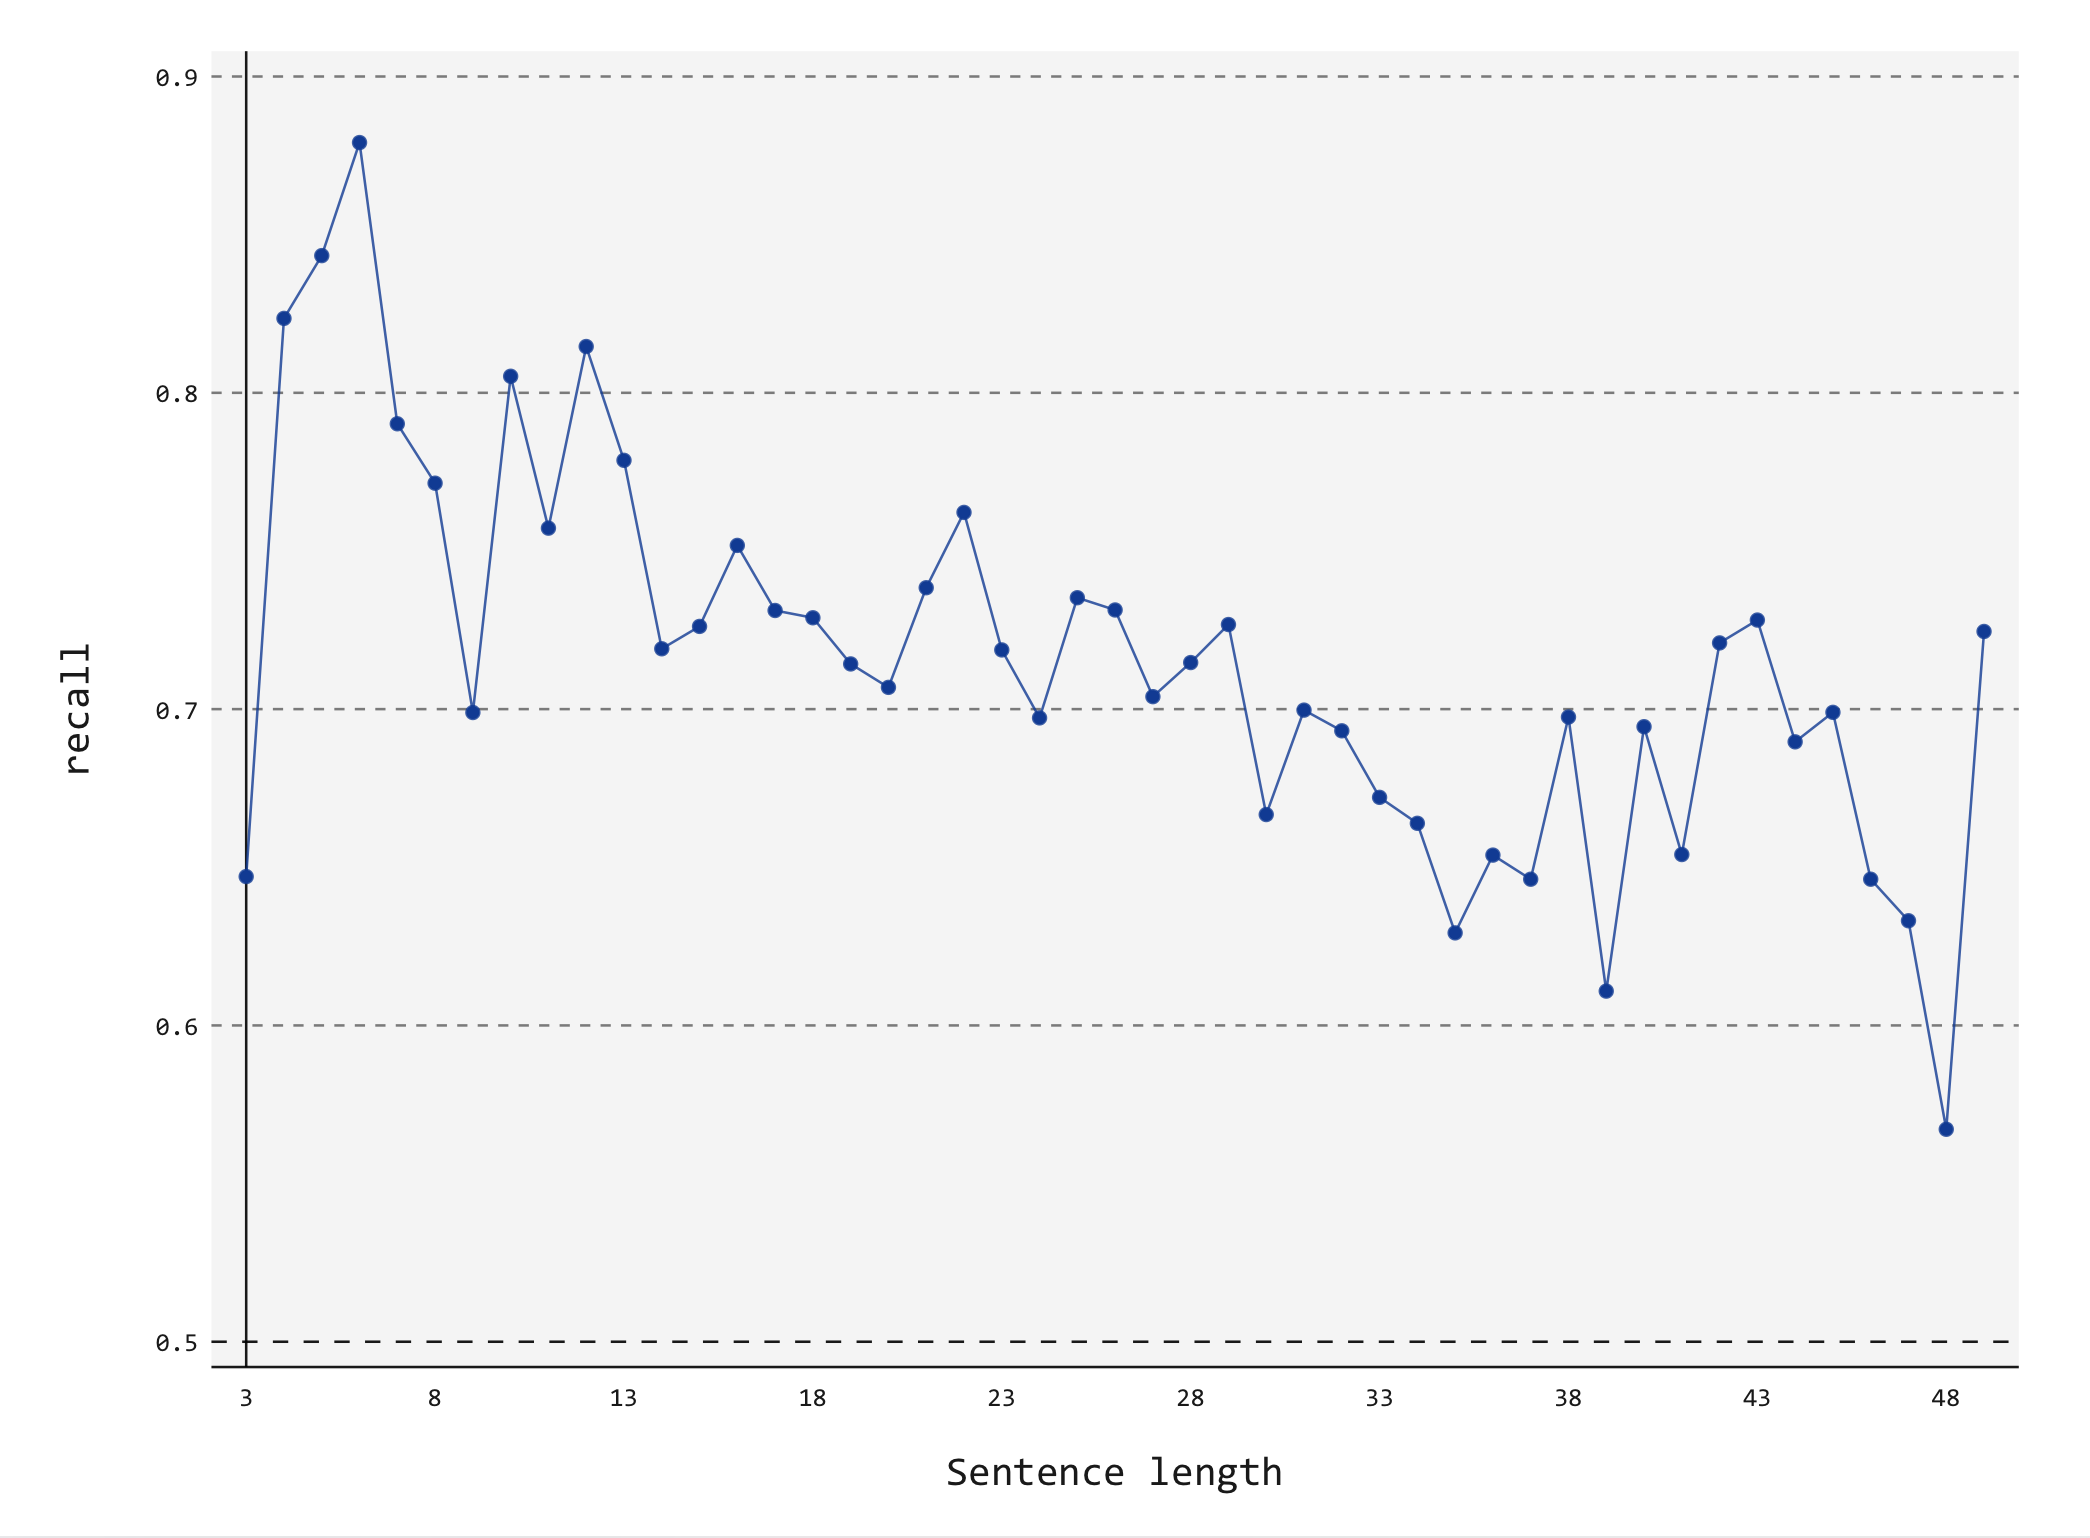
\includegraphics[width=\textwidth]{sentence_psd_turku_recall}
    \end{minipage}
    
    \caption{Labeled precision and recall of the Lisbon (top), Peking (middle), and Turku (bottom) system on the PSD target representation.}
    \label{fig:psd_s_length}
\end{figure}


\subsection{Dependency length}

Another interesting phenomena is the accuracy of a parsing system in relation to dependency length. 


% conclusion
% Both sentence and dependency length have a distribution in the data sets where the frequency of a length factor is correlated with the accuracy for parsing that specific length. The higher the frequency of a given length factor, the more likely that the parsing system has a higher accuracy when parsing a sentence or dependency with a given length. It is therefore important not to exaggerate the importance of the length factor itself, but rather the distribution with which it occurs in the data used for training. So a different data set and distribution would result in, if our assumptions are correct, parsing systems with a different correlation between length and accuracy. 

% However, since we are dealing with natural language, we can also assume that a relatively similar distribution of sentence and dependency lengths observed in the SemEval-2015 data sets will be prevalent in other annotated corpora. We will now turn our attention to specific graph factors, such as distance to root, projectivity, and singletons, and examine the accuracy of the three parsing systems in relation to these aspects of semantic dependency parsing.

\section{Graph factors}
% distance to root
% projectivity
% singletons

\section{Linguistic factors}
% part of speech
% labels

\section{Frames}
% just frames
% complete frames

\section{Conclusions}

In this chapter we have examined the results of Peking, Turku and Lisbon parsing systems as submitted to SemEval-2015. Our examinations have uncovered some interesting phenomena, such as the fact that the overall accuracy of all parsing systems drop in correlation to sentence and dependency length. That the parsing systems are more prone to errors in regards to certain graph and linguistic factors. We have shown that, although some parsing errors can be attributed to lower frequency in the training data, there are also other factors that impact parsing where an increase in training data would not necessarily translate to better results. These type of errors are more related to the technical aspects of the parsing systems themselves. We have seen that different parsing systems produce different types of errors. The results of such an overall analysis could lead the way for ensemble methods where an error analysis is used as basis for weighting.

However, the error analysis did not produce enough evidence to build an overall strategy for improving upon the results of the three semantic dependency parsers examined in this chapter. As mentioned previously, we have instead chosen to focus on improving the accuracy of the classification task of predicting semantic frames. This aspect of semantic dependency parsing is not well researched, and the results of our analysis seem to indicate that there can be room for improvement. In the next chapter we present a set of experiments where we attempt to improve upon the results of SemEval-2015.

% Input for graph images
% \begin{figure}[h]
% \caption{Caption}
% \centering
% 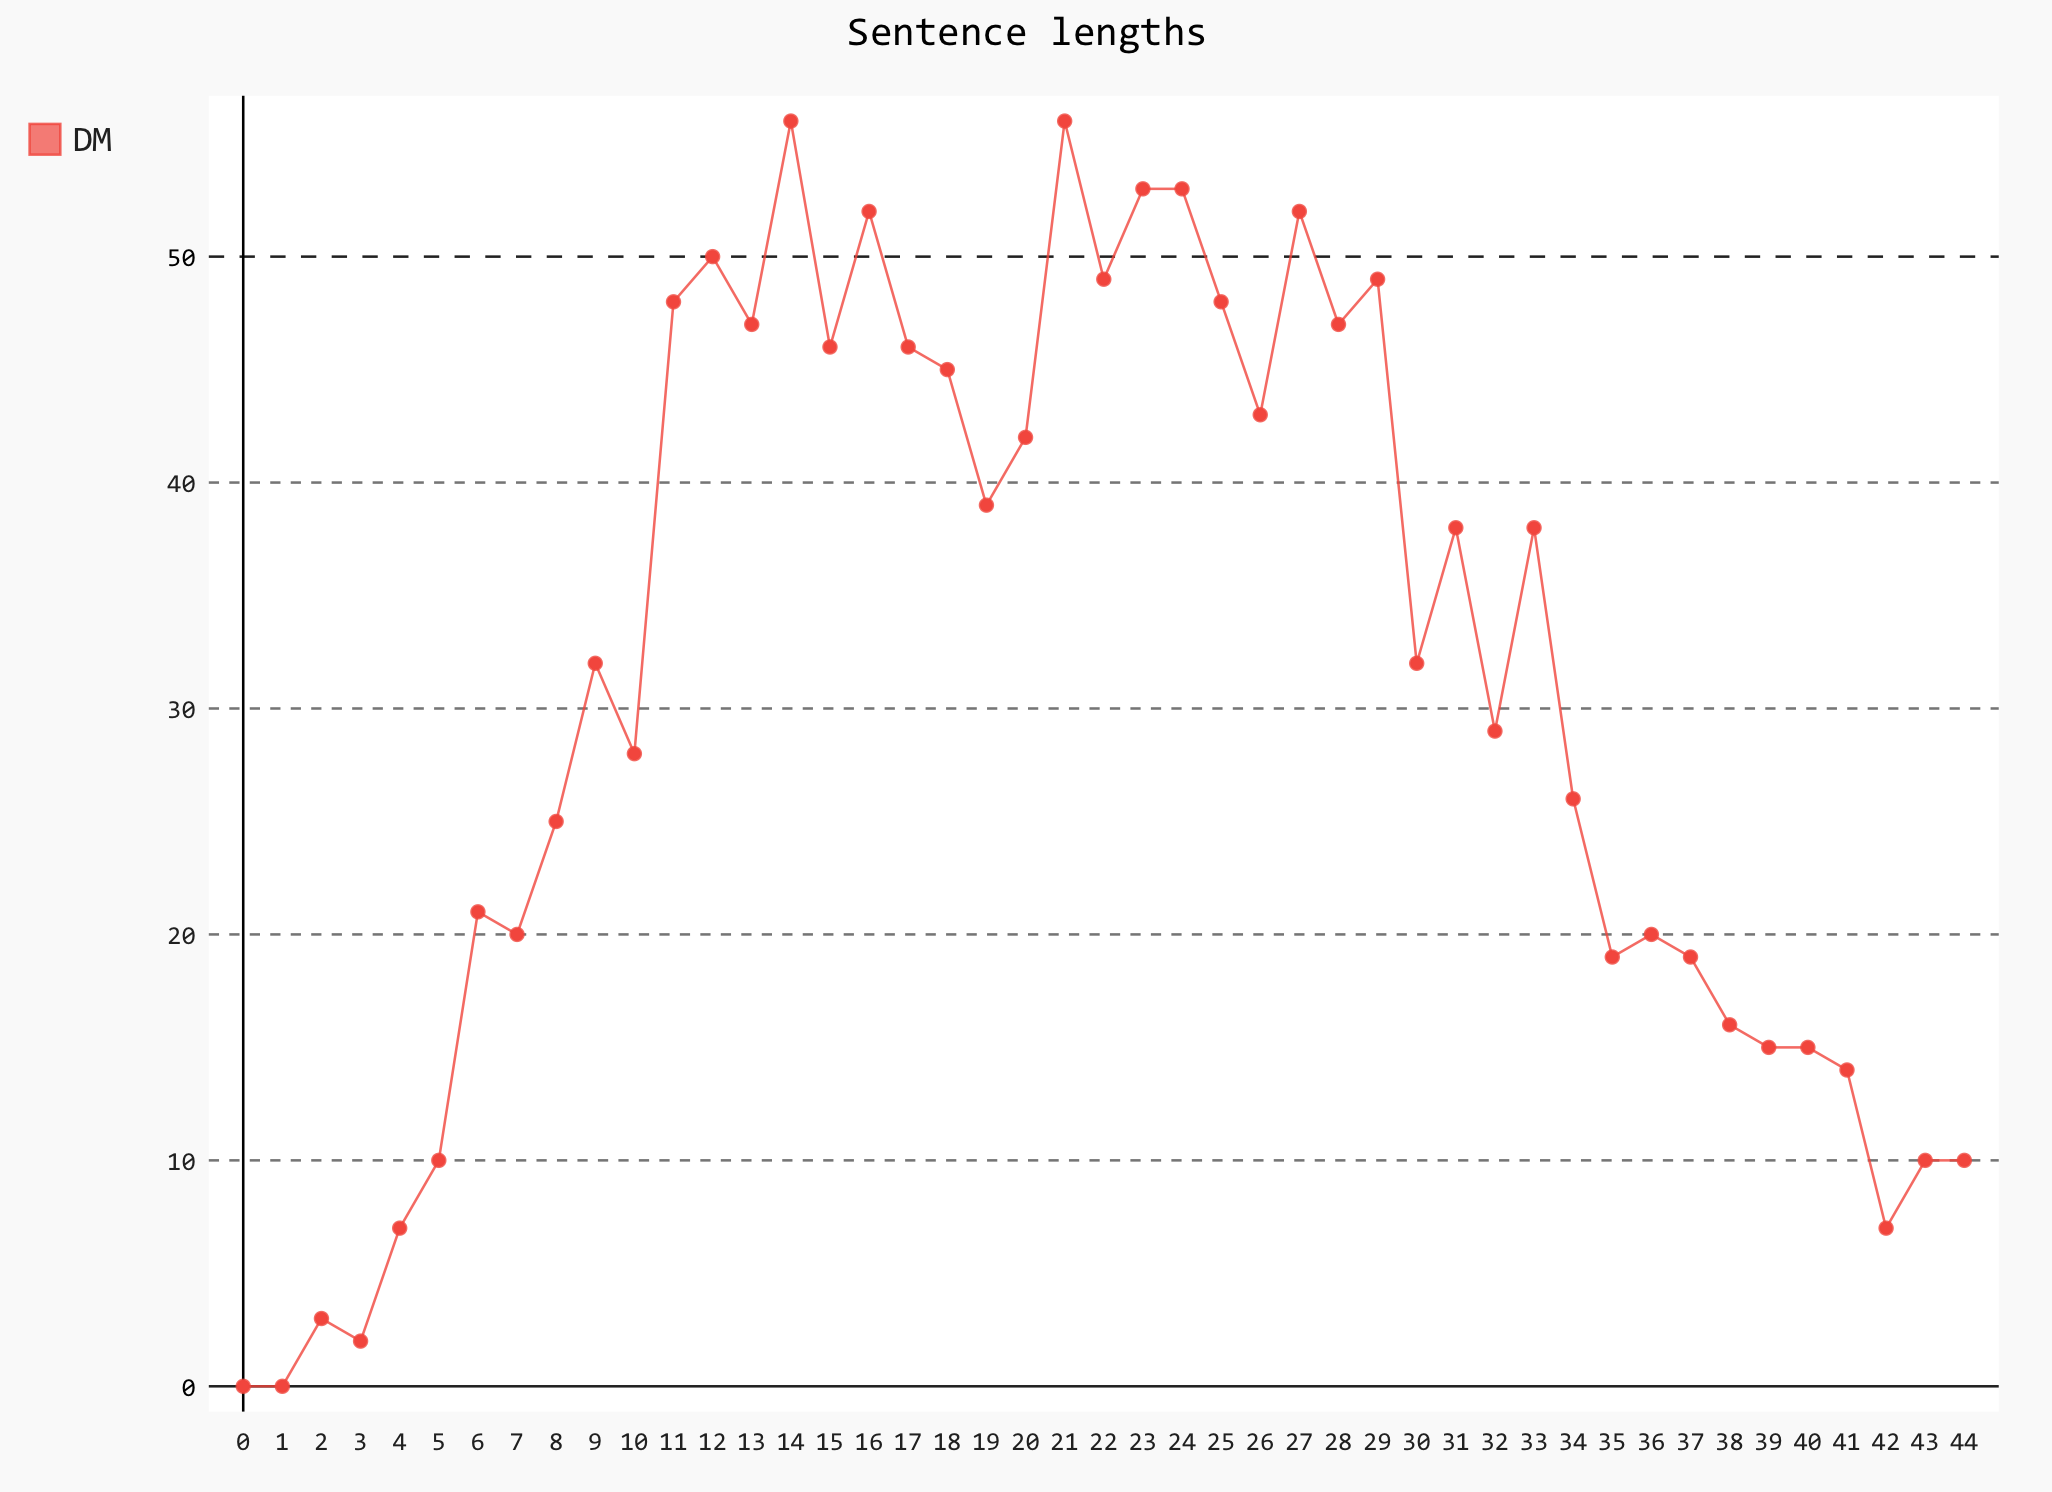
\includegraphics[width=\textwidth]{sentence_length}
% \label{fig:sentence_length}
% \end{figure}